
\documentclass[12pt,letter]{article}
%\documentclass[12pt,letterpaper]{article}

\usepackage{amsmath}
\usepackage{graphics}
\usepackage{graphicx}
\usepackage{epsfig}
\usepackage{fullpage}

%\setlength{\oddsidemargin}{0in}
%\setlength{\evensidemargin}{0in}
%\setlength{\topmargin}{0in}
%\setlength{\headheight}{0in}
%\setlength{\headsep}{0in}
%\setlength{\textheight}{9in}
%\setlength{\textwidth}{6.5in}


\newenvironment{codeblockleft}{\begin{minipage}{6in}\ttfamily\begin{tabbing}}{\end{tabbing}\end{minipage}}

\newenvironment{codeblock}{\begin{center}\begin{codeblockleft}}{\end{codeblockleft}\end{center}}

\newcommand{\boxheader}[1]{\vspace{1.5ex}\pagebreak[1]\noindent\fbox{#1}\vspace{0.8ex}\\}

\newcommand{\method}[1]{\boxheader{\texttt{#1}}}

%% \newcommand{\paramtemplate}[5]{
%% ~\\
%% \noindent\fbox{\texttt{#1}}\\
%% \mbox{\begin{tabular}{ll}
%% Layer:& #2\\
%% Datatype:&\texttt{#3}\\
%% Default value:&#4 #5
%% \end{tabular}
%% }\vspace{1ex}\\}

\newcommand{\paramtemplate}[5]{
~\\
\noindent
\begin{minipage}{\textwidth}
\fbox{\texttt{#1}}\\
\begin{tabular}{ll}
Layer:& #2\\
Datatype:&\texttt{#3}\\
Default value:&#4 #5
\end{tabular}
\end{minipage}
\vspace{0.1ex}\\}


\newcommand{\pparamc}[4]{\paramtemplate{#1}{Parallel only}{#2}{#3}{\\Constraints:&#4}}

\newcommand{\pparam}[3]{\paramtemplate{#1}{Parallel only}{#2}{#3}{}}

\newcommand{\sparamc}[4]{\paramtemplate{#1}{Serial and parallel}{#2}{#3}{\\Constraints&#4}}

\newcommand{\sparam}[3]{\paramtemplate{#1}{Serial and parallel}{#2}{#3}{}}

\newcommand{\groupparams}{\hspace*{\fill}

\vspace{-3.5ex}
}


\begin{document}


\title{
PEBBL 1.0 User Guide
}

\author{
Jonathan Eckstein\thanks{
Business School and RUTCOR, Rutgers University,
640 Bartholomew Road, Piscataway, NJ 08854-8003
}
\and
Cynthia A. Phillips\thanks{
Sandia National Laboratories, Mail Stop 1110, P.O. Box
5800, Albuqurque, NM 87185-1110}
\and
William E. Hart$^{\dagger}$
}

\maketitle

\begin{abstract}
This document describes the UTILIB software library.  UTILIB includes a
variety of generic components for C++ software development including
abstract data types, I/O management, sorting routines, and random number
generators.  The UTILIB library is a core component of the Acro optimization
framework, and it has been used separately for other projects at Sandia,
including DAKOTA and NETV.

\end{abstract}

\newpage

\tableofcontents

\newpage

\section{Introduction}

The Acro Project is an effort to facilitate the design, development, integration and support of optimization software libraries. The goal of the Acro project is to develop optimization solvers and libraries using object-oriented software frameworks that facilitate the application of these solvers to large-scale engineering and scientific applications. Thus Acro includes both individual optimization solvers as well as optimization frameworks that provide abstract interfaces for flexible interoperability of solver components.

This document describes the Acro command line interface (ACLI), which provides a mechanism for defining and solving optimization problems with a general XML syntax.  The goal of the ACLI is to provide a simple, flexible interface for the optimization solvers in Acro. Acro integrates a variety of optimization software packages, including both libraries developed at Sandia National Laboratories as well as publicly available third-party libraries. Thus, the ACLI provides a single framework that supports a wide range of optimization methods. This interface is designed to be easy for users.  Further, the XML driver syntax provides generic mechanisms that should simplify the integration of the ACLI into third-party applications.

The ACLI is designed to be used in two different ways: (1) as an AMPL solver interface, and (2) as an interface for external applications. The next sections describe these usage models and provide examples for the use of ACLI. The remainder of this document describes the XML syntax used to drive ACLI (outside of AMPL).  This XML syntax allows the user to define, reformulate and solve optimization problems.



\section{Downloading and Compiling PEBBL}
\label{sec:downloadcompile}
The PEBBL software project is supported by the Acro optimization
project.  Acro supports the integration of PEBBL builds with auxiliary
libraries, like UTILIB.  PEBBL in turn supports other Acro projects,
such as PICO.

Compiling PEBBL requires a unix-like environment such as Linux or the
Cygwin Linux emulator for Microsoft Windows.  This guide assumes basic
familiarity with the command-line interface to such environments.

The instructions below describe how to download and compile PEBBL and
a minimal set of supporting packages, collectively referred to as
\texttt{acro-pebbl}.  You may also download and compile PEBBL as a
component of larger packages such as PICO; to do so, see the
documentation for those packages.


\subsection{Downloading PEBBL}
\label{sec:download}
You may obtain PEBBL in two ways, either by a conventional tarball or
via the Subversion (\texttt{svn}) version control system.  

\subsubsection{Tarball method}
To obtain a tarball of PEBBL, fill in the form and follow the
instructions on the webpage
\begin{center}
\url{https://software.sandia.gov/trac/acro/wiki/Downloads}
\end{center}
You should uncompress and unbundle the resulting downloaded file, for
example via the command \texttt{tar -xzvf} \emph{filename}.  This
operation should yield a directory named \texttt{acro-pebbl}.

\subsubsection{Subversion method}
Downloading via Subversion will allow you to efficiently track
day-to-day changes in the most recent ``trunk'' version of PEBBL, and
(with permission of the PEBBL team) to more easily contribute changes
and enhancements to the PEBBL source code.

The Subversion method requires that you have both Subversion and the
Python language installed on your system.  First, download the Python
script \texttt{svn.a} from
\begin{center}
\url{https://software.sandia.gov/svn/public/acro/acro-root/trunk/bin/svn.a}
\end{center}
Next, execute the \texttt{svn.a} script with the arguments
\texttt{checkout acro-pebbl}; for example, if you stored
\texttt{svn.a} in your path, you would execute the command
\begin{codeblock}
   svn.a checkout acro-pebbl
\end{codeblock}
As with the tarball method, the end result should be a directory named
\texttt{acro-pebbl}.


\subsection{Compiling: Configuring and Building}
\label{sec:compile}
\label{sec:compiling}
To configure and build PEBBL, enter the \texttt{acro-pebbl} directory
(using \texttt{cd acro-pebbl}, for example).  Then issue the
following commands:
\begin{codeblock}
./setup \\
autoreconf -i -f \\
./configure \textrm{[\emph{options}]} \\
\textrm{[}make clean\textrm{]} \\
make
\end{codeblock}
Note that to configure PEBBL, your system must have \texttt{autoconf}
installed.  The \emph{options} after \texttt{./configure} may be
omitted; if so, you will get a default configuration that effectively
compiles only PEBBL's serial layer (see Section~\ref{sec:arch}).  See
Section~\ref{sec:confopts} below for a description of the possible
configuration options.  The \texttt{make clean} step is only required
if you already configured PICO in the same directory, but have changed
your system configuration or the arguments to \texttt{./configure}.
If you do not need any options to \texttt{./configure}, you may
replace the four-command sequence above with the simple command
\begin{codeblock}
./setup configure make
\end{codeblock}
This method is ``quiet'', redirecting all configuration and
compilation output to the \texttt{test} subdirectory of
\texttt{acro-pebbl}, in the files
\begin{center}
\begin{tabular}{ll}
   \texttt{config.out} & The output of \texttt{autoreconf} 
                         and \texttt{configure} \\
   \texttt{config.xml} & Summary of \texttt{config.out} to detect errors\\
   \texttt{build.out} & The output of \texttt{make}\\
   \texttt{build.xml} & Summary of \texttt{build.out} to detect errors\\
\end{tabular}
\end{center}


\subsubsection{Options for \texttt{configure}}
\label{sec:configoptions}
\label{sec:confopts}
A full list of the possible configuration options may be be obtained
by executing
\begin{codeblock}
configure --help
\end{codeblock}
Some of the more common options are as follows:
\begin{description}
\item[\texttt{--enable-validating}] ~ \\
Increase internal error checking, with a slight performance and
executable size penalty.  
\item[\texttt{--with-debugging}] ~ \\
Compile with additional debug printout capabilities and symbol table
information for stack traces and system debugging tools.  There may
be slight performance and executable size penalty.
\item[\texttt{--without-optimization}] ~ \\
Disable compiler optimization; yields faster compilation at the cost
of slower execution and larger executable files.
\item[\texttt{--with-mpi-compilers=yes}] ~ \\
Enable MPI and the parallel layer, using MPI compilers found in the
current shell path.
\item[\texttt{--with-mpi-compilers=}\textmd{\emph{pathname}}] ~ \\ Enable MPI
and the parallel layer, using MPI compilers installed at
\emph{pathname}.
\end{description}


\section{Architecture and Features}
\label{sec:arch}

PEBBL consists of two \emph{layers}, the \emph{serial layer} and the
\emph{parallel layer}.  The serial layer provides an object-oriented
means of describing branch-and-bound algorithms, with very little
reference to parallel implementation.  If you do not need parallelism,
or are simply in the early stages of algorithm development, the serial
layer allows branch-and-bound methods to be described, debugged, and
run in a familiar, serial programming environment.

The parallel layer contains the core code necessary to create parallel
versions of serial applications.  To parallelize a branch-and-bound
application developed with the serial layer, you simply define
new classes derived from \emph{both} the serial application and the parallel
layer.  A fully-operational parallel application only requires the
definition of a few additional methods for these derived classes,
principally to tell PEBBL how to pack application-specific problem and
subproblem data into MPI message buffers, and later unpack them.

Any parallel PEBBL application constructed in this way inherits the
full capabilities of the parallel layer, including a wide range of
different parallel work distribution and load balancing strategies,
and user-configurable levels of interprocessor communication.  You can
then add application-specific refinements to the parallelization, but
are not required to. Figure~\ref{fig:layers} shows the conceptual
relationship between the two layers, a serial application, and its
parallelization.  In the figure, the application is one of the
examples distributed with PEBBL, for solving binary knapsack problems;
the same basic pattern applies to all PEBBL applications.  The serial
layer class implementing the branch and bound algorithm is called
\texttt{binaryKnapsack}, and the parallel application is called
\texttt{parallelBinaryKnapsack}.  The ``diamond'' inheritance
structure shown in Figure~\ref{fig:layers} is integral to PEBBL's
design --- it is a powerful but sometimes problematic use of C++
multiple inheritance.

\begin{figure}[tpb]
\begin{center}
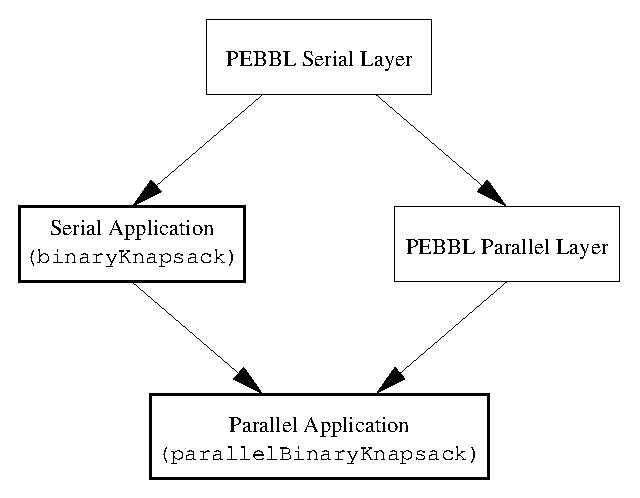
\includegraphics[width=\textwidth]{layers}
\vspace{-0.4in}
\end{center}
\caption{The conceptual relationships of PEBBL's serial layer, the
parallel layer, a serial application (in this case,
\texttt{binaryKnapsack}), and the corresponding parallel application
(in this case, \texttt{parallelBinaryKnapsack}).
\label{fig:layers}
}
\end{figure}


%% \subsection{The knapsack example}
%% This guide will use the binary knapsack problem as an example: given
%% $n$ items each with weight $w_i$ and value $v_i$, $i=1,\ldots,n$, find
%% a ``knapsack''or subset of items of maximum total value whose total
%% weight is less than some given value $C$.  Defining a variable $x_i$
%% to be $1$ if item $i$ is included in the subset, and $0$ otherwise,
%% this problem may be written
%% $$
%% \begin{array}{lll}
%% \max & \sum_{i=1}^n v_i x_i \\
%% \text{S.T.} & \sum_{i=1}^n w_i x_i \leq C \quad\quad \\
%% & x_i \in \{0,1\} & i=1,\ldots,n
%% \end{array}
%% $$ 
%% A simple upper bound on this problem may be computed as follows:
%% sort the items by decreasing $v_i/w_i$ and insert them into the
%% knapsack until no more will fit.  ADD MORE STUFF HERE.......


\subsection{Serial layer architecture}

\subsubsection{The \texttt{branching}, \texttt{branchSub}, 
               and \texttt{solution} classes}

To define a serial branch-and-bound algorithm, you must extend the two
or three key classes in the PEBBL serial layer, \texttt{branching},
\texttt{branchSub}, and possibly \texttt{solution}.  The
\texttt{branching} class stores global information about a problem
instance, and contains methods that implement various kinds of serial
branch-and-bound algorithms, as described below.  Each
\texttt{branchSub} object stores data about a subproblem (or node) in the
branch-and-bound tree, and the \texttt{branchSub} class contains
methods that perform generic operations on subproblems.  The
\texttt{solution} class stores a description of a feasible solution to
the problem.  PEBBL provides some standard \texttt{solution}-derived
template classes, essentially representing solutions as vectors of
standard C++ types such as \texttt{int} or \texttt{double}; for other
solution representations, users should create their own classes
derived from \texttt{solution}.  The basic
\texttt{branching}-\texttt{branchSub}-\texttt{solution} organization
of PEBBL is inspired by ABACUS~\cite{JT98}, but is more general, since
there is no assumption that cutting planes or linear programming are
involved.

By way of example of PEBBL's class structure,
our binary knapsack solver defines a class 
\texttt{binaryKnapsack}, derived from \texttt{branching}, to describe the
capacity of the knapsack and the possible items to be placed in it. We
also define a class \texttt{binKnapSub}, derived from
\texttt{branchSub}, which describes the status of the knapsack items
at nodes of the branching tree (\emph{i.e.}, included, excluded, or
undecided); this class describes a node of the branch-and-bound tree.
Each object in a subproblem class like \texttt{binKnapSub} contains a
pointer back to the corresponding instance of the ``global'' problem
class, in this case \texttt{binaryKnapsack}.  Through this pointer,
each subproblem object can find global information about the problem
instance and the overall
branch-and-bound process.  The knapsack application also defines a
class \texttt{binKnapSolution} derived from \texttt{solution}, to
represent solutions in a compact form that is particularly efficient
for large knapsack problems.

Both \texttt{branching} and
\texttt{branchSub} are derived from a common base class,
\texttt{pebblBase}, which mainly contains common symbol
definitions. The \texttt{branching} class also derives from
\texttt{pebblParams}, which holds command-line-specifiable
parameter objects implemented using the UTILIB class parameter
package.  The \texttt{solution} class also derives from
\texttt{pebblBase}.   Figure~\ref{fig:globalsub} illustrates the basic class
hierarchy for a serial PEBBL application.

\begin{figure}[tbp]
\begin{center}
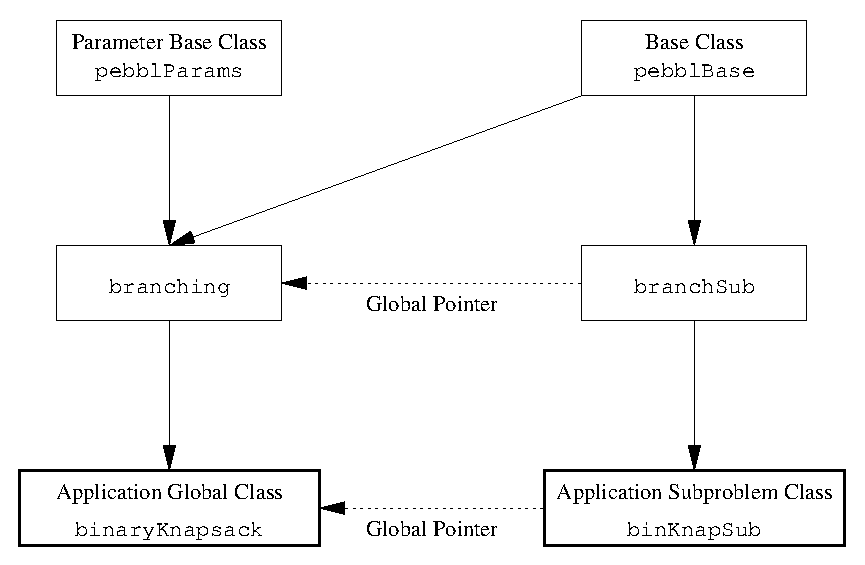
\includegraphics[width=\textwidth]{globalsub}
\vspace{-0.5in}
\end{center}
\caption{Basic class hierarcy for a serial PEBBL application (in this
case, 
\texttt{binaryKnapsack}, with corresponding subproblem class
\texttt{binKnapSub} and solution class \texttt{binKnapSolution}).}
\label{fig:globalsub}
\end{figure}

The class header file for the serial binary knapsack example is in
\url{acro-pebbl/packages/pebbl/src/example/pebbl/serialKnapsack.h}. Note that
\texttt{binaryKnapsack} is defined via
\begin{codeblock}
class binaryKnapsack : virtual public branching \{ $\cdots$ \}
$\;,$
\end{codeblock}
\texttt{binKnapSub} is defined via
\begin{codeblock}
class binKnapSub : virtual public branchSub $\cdots$ \{ $\cdots$ \}
$\;,$
\end{codeblock}
and \texttt{binKnapSolution} is defined via
\begin{codeblock}
class binKnapSolution : public solution $\cdots$ \{ $\cdots$ \} $\;.$
\end{codeblock}
In order for subsequent parallization to work properly, you should use
\texttt{virtual} when deriving classes from \texttt{branching} and
\texttt{branchSub}.  It is typically not necessary to use
\texttt{virtual} when deriving classes from \texttt{solution}.

Calculations made for subproblems frequently require data
stored in the problem description class, which are accessible via
pointers as depicted by the two horizontal dotted arrows in
Figure~\ref{fig:globalsub}.  To implement the upper arrow, the
definition of the subproblem class must instantiate the abstract
method \texttt{bGlobal()}; in \texttt{binKnapSub}, for example, this
capability is implemented via:
\begin{codeblock}
pro\=tected: \\
\>  binaryKnapsack* globalPtr;\\
public:\\
\>  inline binaryKnapsack* global() const \{ return globalPtr; \};\\
\>  branching* bGlobal() const \{ return global(); \};\\
\end{codeblock}
This pattern should be fairly typical: each object of the
\texttt{branchSub}-derived class should contain a pointer to the
\texttt{branching}-derived object for which it represents a
subproblem.  The \texttt{bGlobal()} method should then be implemented
by casting this pointer to a \texttt{branching*}.


\subsubsection{Manipulating subproblem states}
A key feature of PEBBL, first published in Eckstein et al.~\cite{EPH00}, is that
subproblems remember their \emph{state}.  Each subproblem progresses
through as many as six of these states, \texttt{boundable},
\texttt{beingBounded}, \texttt{bounded}, \texttt{beingSeparated}, 
\texttt{separated}, and \texttt{dead}, as illustrated in
Figure~\ref{fig:states}.

\begin{figure}[tbp]
\begin{center}
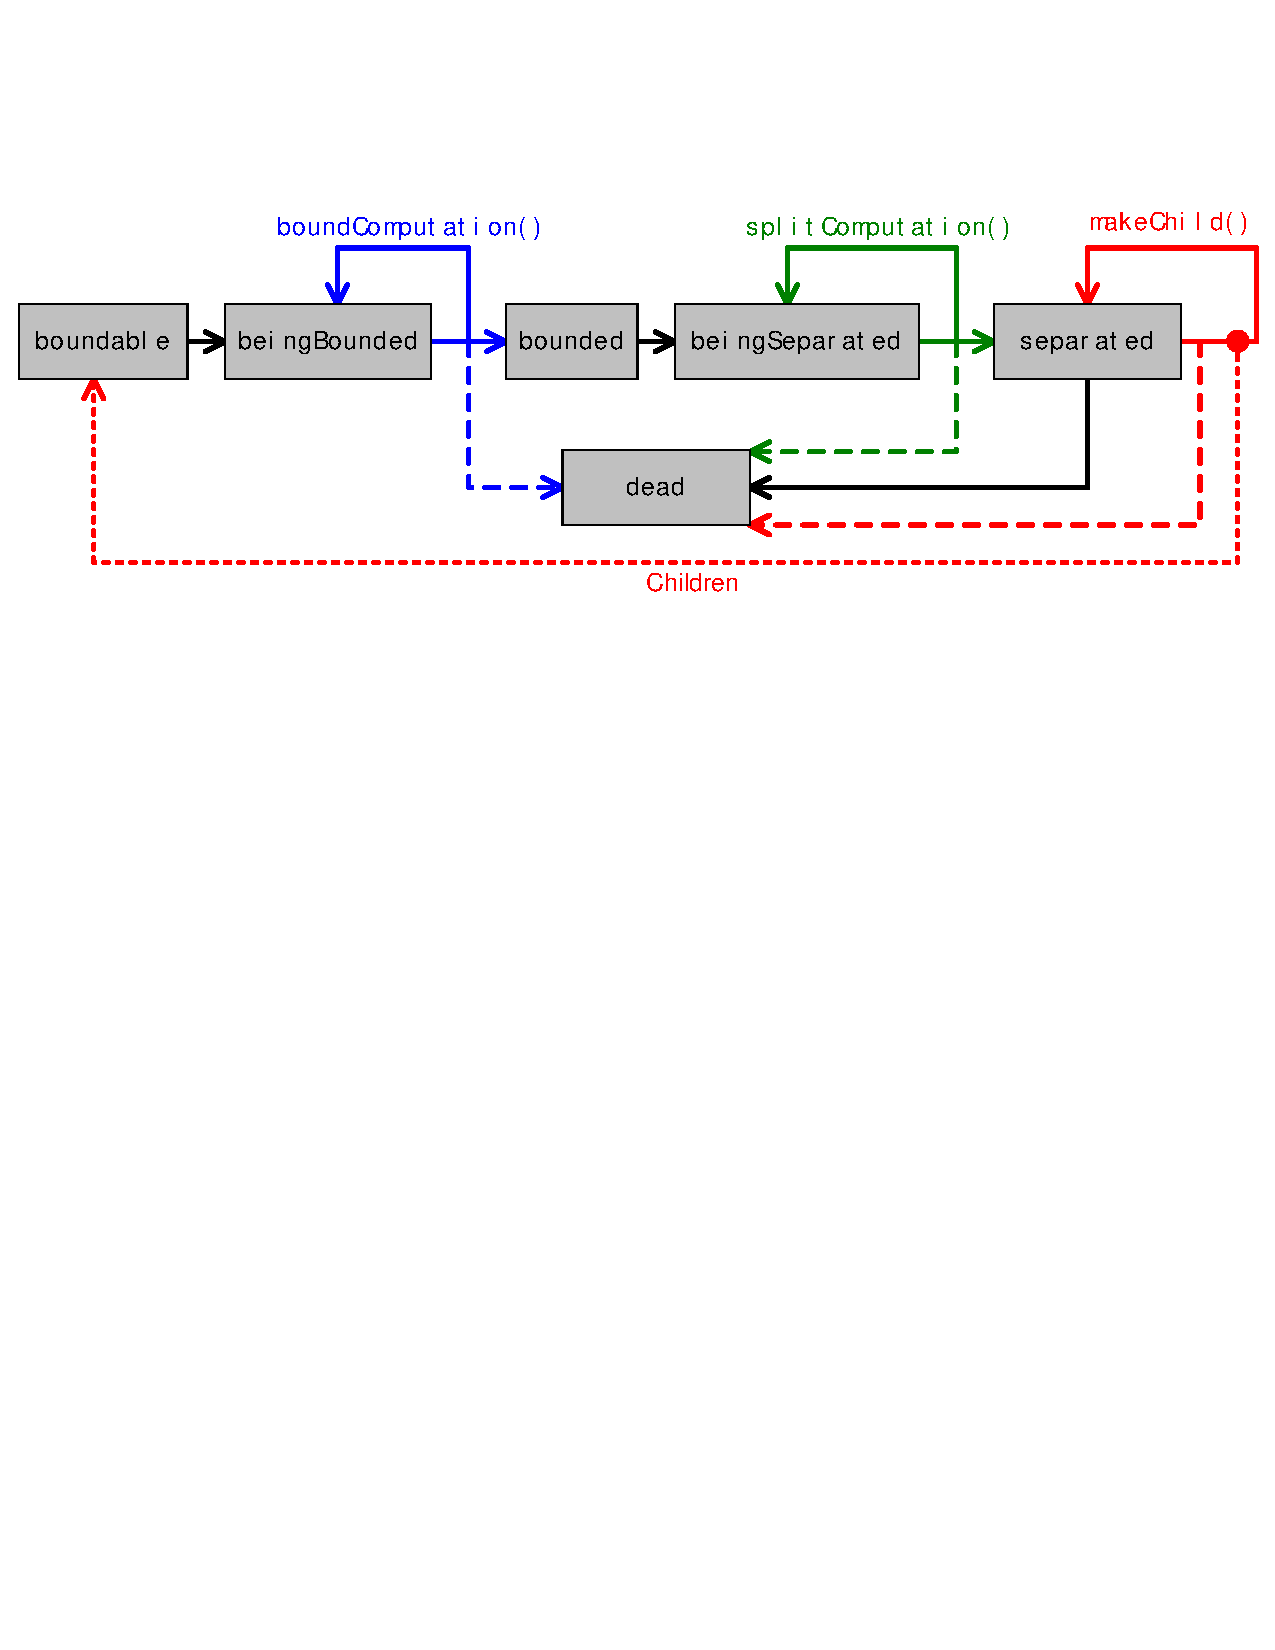
\includegraphics[width=\textwidth]{states-horizontal}
\vspace{-0.5in}
\end{center}
\caption{PEBBL's subproblem state transition diagram.  It is possible
that a single application of \texttt{boundComputation} may take a
subproblem from the \texttt{boundable} state, through
\texttt{beingBounded}, to \texttt{bounded}.  Similarly, a single use
of \texttt{splitComputation} may move a subproblem from
\texttt{bounded}, through \texttt{beingSeparated}, to
\texttt{separated}.}
\label{fig:states}
\end{figure}

A subproblem always comes into existence in state \texttt{boundable},
meaning that little or no bounding work has been done for it, although
it still has an associated bound value; typically, this bound value is
simply inherited from the parent subproblem.  Once PEBBL starts work on
bounding a subproblem, its state becomes \texttt{beingBounded}, and
when the bounding work is complete, the state becomes
\texttt{bounded}.

Once a problem is in the \texttt{bounded} state, PEBBL may elect to
split it into smaller subproblems.  At this point, the subproblem's
state becomes \texttt{beingSeparated}.  Once separation is complete,
the state becomes \texttt{separated}, at which point the subproblem's
children may be created.  Once the last child has been created, the
subproblem's state becomes \texttt{dead}, and it may be deleted from
memory.  Subproblems may also become \texttt{dead} at earlier points
in their existence, because they have been fathomed or represent
portions of the search space containing no feasible solutions.

Class \texttt{branchSub} has three key abstract virtual methods,
namely \texttt{boundComputation}, \texttt{splitComputation}, and
\texttt{makeChild}, that are responsible for applying these state
transitions to subproblems.  PEBBL's search framework interacts with
applications primarily through these methods; defining a PEBBL
branch-and-bound application essentially consists of providing
definitions for these three operators for the application subproblem
class ({\em e.g.} \texttt{binKnapSub}).

The \texttt{boundComputation} method's job is to move the subproblem
to the \texttt{bounded} state, updating the data member \texttt{bound}
to reflect the computed bound value.  The \texttt{boundComputation} method
is allowed to pause an indefinite number of times, leaving the
subproblem in the \texttt{beingBounded} state.  The only requirement
is that any subproblem will eventually become \texttt{bounded} after
some finite number of applications of \texttt{boundComputation}.  This
flexibility allows PEBBL to support branch-and-bound variants where 
bounding is suspended on a subproblem, the subproblem is set aside, and another
task or subproblem is considered.  It also allows for bounding
procedures that establish progressively stronger bounds through
multiple stages of computation.  The
subproblem's bound, reflected in the data member \texttt{bound}, may
change at each step of this process.  When \texttt{boundComputation}
decides that there is no more bounding work to be done for subproblem,
it should change the subproblem state to bounded by executing
\texttt{setState(bounded)}.  Changes in subproblem state should be
implemented via the \texttt{setState} rather than by direct assignment
to the data member \texttt{state} to ensure PEBBL can keep accurate
subproblem statistics.

The \texttt{splitComputation} method's job is similar to
\texttt{boundComputation}'s, but it manages the process of splitting
subproblems.  Eventually it must execute \texttt{setState(separated)}
to signal that the subproblem is completely separated, and then return
the number of child subproblems (\texttt{splitComputation} has a
return type of \texttt{int}).  Before that, however, it is allowed to
return an indefinite number of times with the problem left in the
\texttt{beingSeparated} state (in which case the return value is
ignored).  
This feature allows PEBBL to implement
branch-and-bound methods where the work in separating a subproblem is
substantial and might need to be paused to attend to some other
subproblem or task.  The subproblem's bound may be updated by
\texttt{splitComputation} if the separation process yields additional
bounding information.

Finally, \texttt{makeChild} returns a \texttt{branchSub*} pointing to
a single child of the subproblem it is applied to.  This parent must
be in the \texttt{separated} state.  After its last child has been
made, PEBBL automatically puts the subproblem in the \texttt{dead}
state.

If at any point in \texttt{boundComputation},
\texttt{splitComputation}, or \texttt{makeChild}, it becomes evident
that a subproblem does not require further investigation --- for
example, because it has become evident the subproblem is infeasible
--- one may mark the subproblem as \texttt{dead} by executing
\texttt{setState(dead)}.

In addition to \texttt{boundComputation}, \texttt{splitComputation},
and \texttt{makeChild}, some additional virtual methods must to be
defined to complete the specification of a branch-and-bound
application; all these methods are described in
Section~\ref{sec:serialMethods}.


\subsubsection{Pools, handlers, and the search framework}
\label{sec:framework}

PEBBL's serial layer orchestrates branch-and-bound search through a
module called the ``search framework'', literally,
\texttt{branching::searchFramework}.  The search framework acts as an
attachment point for two user-specifiable objects, a \emph{pool} and
a \emph{handler}, whose combination determines the exact ``flavor''
of branch and bound being implemented.

The pool object dictates how the currently active subproblems are
stored and accessed, which effectively determines the branch-and-bound
search order.  Currently, there are three kinds of pool: a heap sorted
by subproblem bound\footnote{Objects of type \texttt{branchSub} have a
member called \texttt{integralityMeasure} which may be used by the
application to measure how far a subproblem is from being completely
feasible (that is, from having \texttt{candidateSolution} yield
\texttt{true}; see Section~\ref{sec:serialMethods}).  If two
subproblems have identical bounds, the one with the lower
\texttt{integralityMeasure} will be placed higher in the heap, since
it presumably is more likely to lead to an improved incumbent
solution.}, a stack, and a FIFO queue.  If you specify the heap
pool, then PEBBL will follow a best-first search order; specifying the
stack pool results in a depth-first order, and specifying the queue
results in a breadth-first order. 

Critically, at any instant in time, the subproblems in the pool may in
principle represent any mix of states: for example, some might be
\texttt{boundable}, and others \texttt{separated}.  This feature gives
you flexibility in specifying the \emph{bounding protocol}, which is a
different aspect of the algorithm than the search order; each
``handler'' object implements a particular bounding protocol.

To illustrate what a bounding protocol is, consider the usual
branch-and-bound method for mixed integer programming as typically
described by operations researchers: one removes a subproblem from the
currently active pool, and computes its linear programming relaxation
bound.  If the bound is strong enough to fathom the subproblem, it is
discarded.  Otherwise, one selects a branching variable, creates two
child subproblems, and inserts them into the pool.  This type of
procedure is an example of what is often called ``lazy'' bounding (see
for instance~\cite{CP99}), because it views the bounding procedure as
something time-consuming (like solving a large linear program) that
should be delayed if possible.  In the PEBBL framework, lazy bounding
is implemented by a handler that tries to keep all subproblems in the
active pool in the \texttt{boundable} state.

An alternative approach, common in work originating from the computer
science community, is usually called ``eager'' bounding (again,
see~\cite{CP99} for an example of this terminology).  Here, all
subproblems in the pool have already been bounded.  One picks a
subproblem out of the pool, immediately separates it,
and then forms and bounds each of its children.  Children whose bounds do
not cause them to be fathomed are returned to the pool.  

Lazy and eager bounding each have their own advantages and
disadvantages, and the best choice may depend on both the application
and the implementation environment.  Typically, implementors seek to
postpone the most time-consuming operations in the hope that the
discovery of a better incumbent solution will make them unnecessary.
So, if the bounding operation is much more time-consuming than
separation, lazy bounding is most appealing.  If the bounding
operation is very quick, but separation more difficult, then eager
bounding would be more appropriate.  Eager bounding may save some
memory since leaf nodes of the search tree may be processed without
entering the pool, but has a larger task granularity, resulting in
lower parallel communication overhead per subproblem, but also
somewhat less potential for parallelism.

\begin{figure}[tbp]
\begin{center}
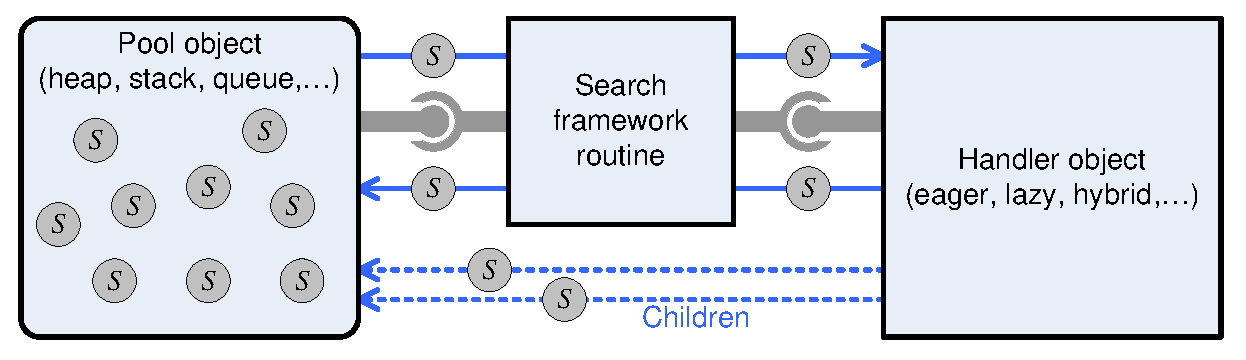
\includegraphics[width=\textwidth]{framework}
\vspace{-0.5in}
\end{center}
\caption{The search framework, pool, and handler.  Each $S$
indicates a branch-and-bound subproblem --- an object of type derived
from \texttt{branchSub}.}
\label{fig:poolandhandler}
\end{figure}

Because PEBBL's serial layer stores subproblem states and lets the
you specify a handler object, it gives you the freedom to specify
lazy bounding, eager bounding, or other protocols.  The search
framework routine simply extracts subproblems from the pool and passes
them to the handler until the pool becomes empty.  Currently, there
are three possible handlers, \texttt{eagerHandler},
\texttt{lazyHandler}, and \texttt{hybridHandler}.  The
\texttt{eagerHandler} and \texttt{lazyHandler} 
objects respectively implement eager
and lazy bounding by trying to keep as many subproblems
as possible in the \texttt{bounded} and \texttt{boundable} states,
respectively.

The \texttt{hybridHandler} object implements a strategy that is somewhere
between eager and lazy bounding, and is perhaps the most simple and
natural given PEBBL's concept of subproblem states.  Given any
subproblem, \texttt{hybridHandler} performs a single application of
either \texttt{boundComputation}, \texttt{splitComputation}, or
\texttt{makeChild}, to try to advance the subproblem one transition
through the state diagram of Figure~\ref{fig:states}.  
If the subproblem's state is
\texttt{boundable} or \texttt{beingBounded}, it applies
\texttt{boundComputation} once.  If the subproblem's state is
\texttt{bounded} or \texttt{beingSeparated}, it applies {\tt
splitComputation} once.  Finally, if the state is \texttt{separated},
the handler performs one call to \texttt{makeChild}, and inserts the
resulting subproblem into the pool.  \texttt{Hybridhandler} is currently
PEBBL's default choice of handler.

The combination of multiple handlers, multiple pool implementations,
and the freedom in implementing \texttt{boundComputation} and
\texttt{splitComputation} create considerable flexibility in the kinds
of branch-and-bound methods that the serial layer can implement.
Figure~\ref{fig:poolandhandler} depicts the relationship of the search
framework, pool, and handler.

You may choose between the existing pools and handlers by setting
parameters in the \texttt{branching} class object; see
Section~\ref{sec:searchparams}.  You may also in principle supply
your own pools and handlers, but we consider that an advanced topic,
and it is not presently covered in this guide.


\subsection{Controlling the Search Process}

\subsubsection{Basic tolerances}

In its normal, non-enumeration 
mode of operation, PEBBL's optimality criteria are
controlled by two parameters, \texttt{absTolerance} and
\texttt{relTolerance}, with respective default values $0$ and
$10^{-7}$. PEBBL attempts to locate a single problem solution that is
either within an additive distance \texttt{absTolerance} or a relative
distance \texttt{relTolerance} of optimality, whichever turns out to
be less restrictive.  For example, setting \texttt{relTolerance} to
$0.05$ would specify a solution with 5\% of optimality.


\subsubsection{Multiple solutions: enumeration criteria
  and the solution repository}

PEBBL can also function in an enumeration mode in which it stores
multiple feasible solutions to a problem.  Enumeration mode is
activated if any of the four parameters \texttt{enumAbsTolerance},
\texttt{enumRelTolerance}, \texttt{enumCutoff} or
\texttt{enumCount} is set.  The meaning of these parameters is as
follows:
\begin{description}
\item[\texttt{enumAbsTolerance}:] Find all solutions whose objective
  value is within \texttt{enumAbsTolerance} of the best possible.  For
  example, setting $\text{\texttt{enumAbsTolerance}}=6$ indicates you
  want all solutions within $6$ units of optimal.
\item[\texttt{enumRelTolerance}:]  Find all solutions within a
  relative distance \texttt{enumRelTolerance} of the best possible.
  For example, setting $\text{\texttt{enumRelTolerance}}=0.10$ specifies
  that PEBBL should enumerate all solutions within $10$\% of optimal. 
\item[\texttt{enumCutoff}:]  Find all solutions with an objective
  value better than this value.  For a minimization problem, for
  example, setting $\text{\texttt{enumCutoff}}=0$ instructs PEBBL to
  find all solutions with a negative objective value.
\item[\texttt{enumCount}:]  Find the best \texttt{enumCount}
  solutions; for example setting $\text{\texttt{enumCount}}=10$
  requires PEBBL to find the $10$ best solutions.
\end{description}

If you set more than one of these parameters, PEBBL returns only
solutions simultaneously meeting all the specified criteria.  For
example, setting $\text{\texttt{enumRelTolerance}}=0.05$ and
$\text{\texttt{enumCount}}=200$ means that PEBBL should return only
those solutions that are among the $200$ best and are also within
$5$\% of optimal.

The enumeration mechanism keeps a repository of feasible solutions
represented as objects of type derived from the \texttt{solution}
class, maintained both as a hash table and heap in reverse order of
solution quality --- that is, the solution on the top of the heap has
the worst objective value.  The hash table representation, along with
hashing and comparison and methods of the \texttt{solution} class,
prevents duplicate solutions from entering the repository.  Discovery
of a new best incumbent solution can cause solutions to be removed
from the repository if either \texttt{enumAbsTolerance} or
\texttt{enumRelTolerance} is set.  If \texttt{enumCount} is set and
the repository already contains \texttt{enumCount} solutions, then
entry of a new solution into the repository causes the previously
worst solution in the repository to be removed.


\subsubsection{The \texttt{solution} class}
\label{sec:solclass}
PEBBL represents optimization problem solutions by objects derived
from the abstract class \texttt{solution}.  PEBBL provides a template
class, \texttt{arraySolution<\emph{T}>}, which represents solutions as a
one-dimensional array or vector of type \texttt{\emph{T}}.  This solution
representation should be adequate for many applications; if it is not
convenient or efficient for a given application, users may create
their own \texttt{solution}-derived classes.  It is even possible for
a single application to use several different solution
representations.

To properly maintain the hash table used to filter out duplication
solutions, PEBBL needs a hash function that may be applied to
solutions, and a means of comparing two solutions to see if they are
duplicates.  The normal means of hashing and comparison are through
the \emph{sequence representation} of solutions.  The
\texttt{solution} class contains abstract methods
\texttt{sequenceLength}, \texttt{sequenceData}, and
\texttt{sequenceReset} whose purpose is to convert a solution to
sequence of \texttt{double}s, in such a way that two solutions may be
considered duplicates if and only if invoking these methods results in identical
behavior.  If these methods are implemented, PEBBL automatically
supplies a hash function in the method \texttt{computeHashValue}, and
comparison operator for solutions is the method \texttt{duplicateOf}.

It is possible to dispense with the sequence representation methods;
in this case, however, users must provide their own explicit
implementations of \texttt{computeHashValue} and
\texttt{duplicateOf}.  Even if a sequence representation is defined,
users might want to override either of these methods in the interest
of efficiency.


\subsubsection{Early output and checkpointing}

Some of the calculations for which PEBBL is intended may be extremely
long-running, and thus vulnerable to data loss if a system crashes
or a job's time allocation is exhausted.  PEBBL has two features
designed to mitigate such data loss.  The first, \emph{early output},
tries to ensure that if a PEBBL run is interrupted, you can recover
the best solution found so far.  You enable this feature by setting
the parameter \texttt{earlyOutputMinutes} to some positive value $m$.
Each time PEBBL finds a new incumbent solution (that is, a solution
better than all previously found ones) that exists for at least $m$
minutes, PEBBL writes it to disk so that it is available if
the run crashes. Early output is also useful if you wish to
voluntarily terminate a run and still have access to the best feasible
solution computed so far.  
This feature may be useful in early testing of an application for which you
may not yet know appropriate tolerance values.  For example, if you initiate
a run with a \texttt{relTolerance} of 5\%, but after considerable computation,
the optimality 
gap is still 10\%, you may decide you are satisfied with the 10\%
tolerance.

The second data loss mitigation feature is \emph{checkpointing}, which
imposes more overhead on PEBBL, but is more powerful.  Checkpointing is
currently available only for the parallel layer; it is not available
in applications built solely on the serial layer.  The key parameter
controlling checkpointing is \texttt{checkPointMinutes}.  If this
parameter has a positive value $m$, PEBBL writes its complete
internal state to disk approximately every $m$ minutes. Each processor
writes a separate file, and the checkpointing feature requires that
all processors have access to file I/O, although not necessarily to the
same directory.

The computation can be restarted from the time of the checkpoint by
specifying either of the command-line parameters \texttt{restart} or
\texttt{reconfigure}.\footnote{As with all PEBBL command-line
  parameters, these parameters should be preceeded by two hyphens when
  used on the command line, as in \texttt{--restart}.} 
Using \texttt{restart} is potentially faster, but
\texttt{reconfigure} allows one to restart with a different parallel
configuration --- for example, a different total number of processors.
To use \texttt{reconfigure}, all checkpoint files must be in (or moved
to) the same directory.

Some MPI implementations provide their own checkpointing capabilities.
PEBBL's checkpointing feature is independent of any such capabilities
and does not require them.  

The early-output mechanism and enumeration mechanisms are
currently independent.  When using enumeration, the early output mechanism
simply outputs the best incumbent.  Checkpointing, however, is fully
compatible with enumerating multiple solutions: each checkpoint will
save the entire state of the solution repository.



\subsection{Parallel layer architecture}

PEBBL's parallel layer attempts to accelerate the branch-and-bound
process by using multiple processors, and requires some form of the
MPI message passing interface.  PEBBL's parallel layer will run on
shared-memory (SMP) systems, but only if MPI is configured to emulate a
message passing environment (which is the default on multicore systems
when packages such as OpenMPI are downloaded with utilities such as
the Ubuntu package manager).  

PEBBL's primary mode of parallelism, as is standard in parallel branch
and bound, is to explore different nodes of the search tree
simultaneously on different processors.  However, PEBBL has the
optional capability to use different modes of parallelism during the
early stages of the search; see Section~\ref{sec:rampup} below.

For the most part, parallel-layer search node processing is carried
out by the same \texttt{boundComputation}, \texttt{splitComputation},
and \texttt{makeChild} methods as in serial layer.  Thus, once you
have created these methods for your application, parallel execution
should be available with little additional development effort.


\subsubsection{Inheritance pattern}

The parallel layer's capabilities are embodied in the classes
\texttt{parallelBranching} and {\tt paral\-lel\-BranchSub}, which have the
same function as \texttt{branching} and \texttt{branchSub},
respectively, except that they perform parallel search of the
branch-and-bound tree.  Both are derived from a common base
class \texttt{parallelPebblBase}, whose function is similar to
\texttt{pebblBase}, containing mainly common symbol definitions.
The class \texttt{parallelBranching} also derives from
\texttt{parallelPebblParams}, which contains a large number of
parameters for controlling parallel search.  Furthermore, each of
\texttt{parallelBranching} and {\tt parallelBranchSub} is derived from
the corresponding class in the serial layer.

To turn a serial application into a parallel application, one must
define two new classes.  The first is derived from
\texttt{parallelBranching} and the serial application global class.
In the knapsack example, for instance, we defined a new class
\texttt{parallelBinaryKnapsack} which has both
\texttt{parallelBranching} and \texttt{binaryKnapsack} as
\texttt{virtual} base classes.  We call this class the \emph{global
parallel class}.  For each problem instance, the information in the
global parallel class is replicated once on every processor.

This basic inheritance pattern is repeated for
parallel subproblem objects.  In the knapsack case, we defined a
parallel subproblem class \texttt{parBinKnapSub} to have
\texttt{virtual} \texttt{public} base classes \texttt{binKnapSub} and
\texttt{parallelBranchSub}.  As with the serial subproblems, each
instance of \texttt{parBinKnapSub} has a
\texttt{parallelBinaryKnapsack} pointer that allows it to locate
global problem information.  Figure~\ref{fig:parinherit} depicts the
inheritance structure for the parallel knapsack application.  The
classes \texttt{solution} and \texttt{binKnapSolution} are omitted
from the figure since their relationship is unchanged from
Figure~\ref{fig:globalsub}, although a few additional \texttt{virtual}
methods in \texttt{solution} may need
to be implemented for parallel operation.

\begin{figure}[tb]
\begin{center}
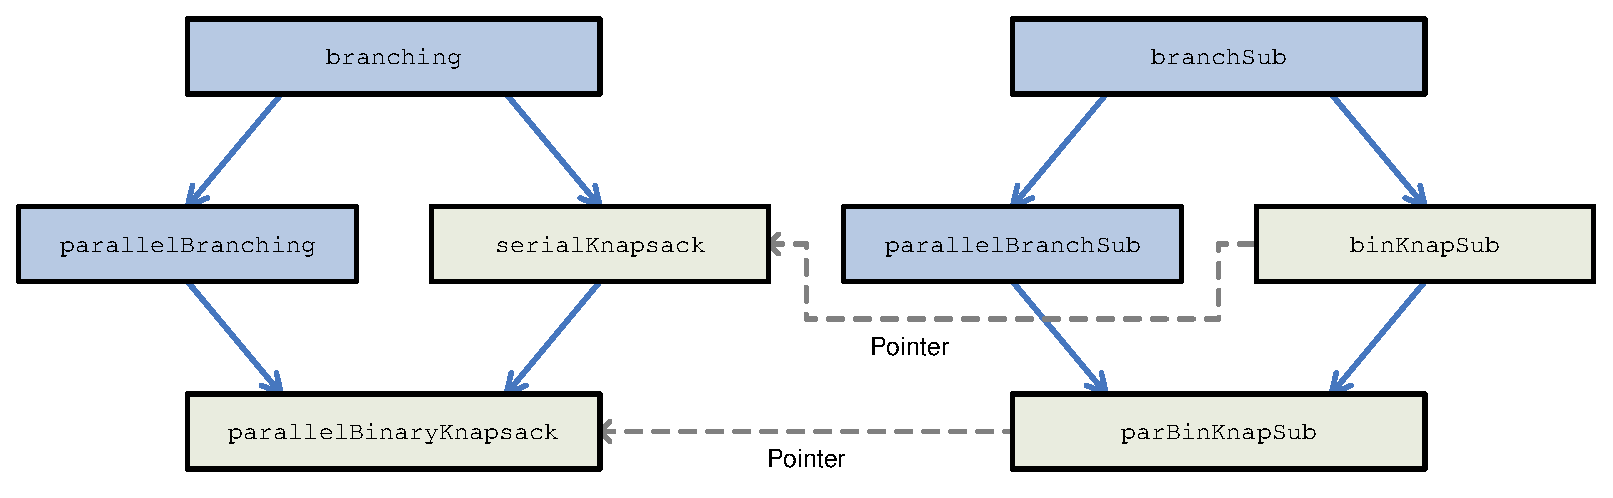
\includegraphics[width=\textwidth]{parinherit-new}
\vspace{-0.4in}
\end{center}
\caption{Partial depiction of the inheritance structure of the
  parallel knapsack application.  Other parallel applications are
  similar.}
\label{fig:parinherit}
\end{figure}

The header file
\url{acro-pebbl/packages/pebbl/src/example/pebbl/parKnapsack.h}
defines the inheritance structure depicted in
Figure~\ref{fig:parinherit}.  It defines
\texttt{parallelBinaryKnapsack} via
\begin{codeblock}
class \=parallelBinaryKnapsack : \\
\>public parallelBranching, \\
\>public binaryKnapsack \\
\{ \\
\>$\vdots$\\
\}$\;,$\\
\end{codeblock}
and \texttt{parBinKnapSub} via
\begin{codeblock}
cla\=ss \=parBinKnapSub : \\
\>\>public parallelBranchSub, \\
\>\>public binKnapSub \\
\{ \\
private: \\
\>parallelBinaryKnapsack* globalPtr; \\
public: \\
\>parallelBinaryKnapsack* global()  const \{ return globalPtr; \}; \\
\>parallelBranching*      pGlobal() const \{ return globalPtr; \}; \\
\>\>$\vdots$\\
\}
\end{codeblock}

Once this basic inheritance pattern is established, the parallel
application automatically combines the description of the application
coming from the serial application (in the knapsack case, embodied in
\texttt{binaryKnapsack} and \texttt{binKnapSub}) with the parallel
search capabilities of the the parallel layer.  For the parallel
application to function, however, additional methods must be defined,
as summarized in Section~\ref{sec:parMethods}.  The most critical of
these methods are \texttt{pack} and \texttt{unpack}, which must be
defined for the global parallel class, the subproblems, and solutions.
These methods respectively describe how to encode and decode objects
into a UTILIB \texttt{Packbuffer} or \texttt{UnPackBuffer}
object (see the UTILIB documentation).
%% For the global parallel class, PEBBL uses
%% \texttt{pack} and \texttt{unpack} when it broadcasts the problem
%% description to all processors at the outset of the parallel search.
%% For subproblems, PEBBL uses \texttt{pack} and \texttt{unpack} in the
%% transmission of subproblems between processors.

\subsubsection{Processor clustering}
\label{sec:clustering}
PEBBL's parallel layer employs a generalized form of the processor
organization used by the later versions of CMMIP~\cite{Eck94,Eck97}.
Processors are organized into \emph{clusters}, each with one
\emph{hub} processor and one or more \emph{worker} processors.  The
hub processor serves as a ``master'' in work-allocation decisions,
whereas the workers are in some sense ``slaves,'' doing the actual
work of bounding and separating subproblems. The degree of control
that the hub has over the workers may be varied by a number of
run-time parameters, and may not be as tight as a classic
``master-slave'' system.  Further, the hub processor has the option of
simultaneously functioning as a worker.

Three run-time parameters, all defined in \texttt{parallelPebblParams},
govern the partitioning of processors into clusters: {\tt
clusterSize}, \texttt{numClusters}, and \texttt{hubsDontWorkSize}.  First
PEBBL finds the size $k$ of a ``typical'' cluster via the formula
\begin{eqnarray*}
k &= &
\min \left\{ 
\mbox{\tt clusterSize},
\max \left\{
\left\lfloor \frac{\overline{p}}{\mbox{\tt numClusters}}
\right\rfloor,
1
\right\}
\right\} ,
\end{eqnarray*}
where $\overline{p}$ is the total number of processors.  Thus, $k$ is
the smaller of the cluster sizes that would be dictated by
\texttt{clusterSize} and \texttt{numClusters}.  Processors are then
gathered into clusters of size $k$, except that if $k$ does not evenly
divide $\overline{p}$, the last cluster will be of size
$\overline{p}\; \mbox{mod}\;k$.
In clusters whose size is greater than or equal to
\texttt{hubsDontWorkSize}, the hub processor is ``pure,'' that is, it
does not simultaneously function as a worker.  In clusters smaller
than \texttt{hubsDontWorkSize}, the hub processor is also a worker.
The rationale for this arrangement is that, in very small clusters,
the hub will be lightly loaded, and its spare CPU cycles should be
used to help explore the branch-and-bound tree.  If a cluster is too
big, however, using the hub simultaneously as a worker may
unacceptably delay the hub's response to messages, slowing down the
entire cluster.  In such cases, a ``pure'' hub is preferable.


\subsubsection{Tokens and work distribution within a cluster}
\label{sec:withincluster}
Unlike some ``master-slave'' implementations of branch and bound, each
PEBBL worker maintains its own pool of active subproblems.  This pool
may be any of the kinds of pools described in
Section~\ref{sec:framework}, although all workers must use the same pool
type.  Depending on various parameter settings, however,
the pool might be very small, in the most extreme case never holding more
than one subproblem.  Each worker processes its pool in the same
general manner as the serial layer: it picks subproblems out of the
pool and passes them to a search handler until the pool is empty.
When running in parallel, handlers have the additional ability to
\emph{release} subproblems from the worker to the hub.

For the remainder of this subsection, assume for simplicity that a
single cluster spans all available processors; in the next subsection,
we will amend our description to cover the case of multiple clusters.

\paragraph{Random release of subproblems:}
When running in a parallel context, \texttt{eagerHandler} decides
whether to release a subproblem as soon as it has become
\texttt{bounded}.  In parallel situations, \texttt{lazyHandler} and
\texttt{hybridHandler} make the release decision when they create a
subproblem.  No matter which handler is used, 
the decision is a random one, with the probability of
release controlled by run-time parameters.  Released subproblems do
not return to the local pool; instead, the worker cedes control over
these subproblems to the hub.  Eventually, the hub may send control of
the subproblem back to the worker, or to another worker.

If the release probability is 100\%, then every subproblem is
released, and control of each subproblem is always returned to the hub at
a some point in its lifetime (at creation for \texttt{lazyHandler}
and \texttt{hybridHandler}, and upon reaching the \texttt{bounded} state
for \texttt{eagerHandler}).  In this case, the hub and its workers
function like a standard ``master-slave'' system.  When the
probability is lower, the hub and its workers are less tightly
coupled.  The release probability is controlled by the run-time
parameters \texttt{minScatterProb}, \texttt{targetScatterProb}, and
\texttt{maxScatterProb}.  The use of three different parameters,
instead of a single one, allows the release probability to be
sensitive to a worker's load.  Basically, if the worker appears to
have a fraction $1/w(c)$ of the total work in the cluster, $w(c)$
denotes the total number of workers in 
cluster $c$, then the worker uses the value \texttt{targetScatterProb}.
If it appears to have less work, then a smaller value is used, but no
smaller than \texttt{minScatterProb}; if it appears to have more work,
it uses a larger value, but no larger than \texttt{maxScatterProb}.

\paragraph{Subproblem tokens:}
When a subproblem is released, only a small portion of its data,
called a \emph{token}~\cite{RRM93,Eck94}, is actually sent to the hub.
The subproblem itself may move to a secondary pool, called the
\emph{server pool}, that resides on the worker.  A token consists of
only the information needed to identify a subproblem, locate it in the
server pool, and schedule it for execution.  Since the hub receives
only tokens from its workers, as opposed to entire subproblems, these
space savings translate into reduced storage requirements and
communication load at the hub.

When making tokens to represent new, \texttt{boundable} subproblems,
the parallel version of \texttt{lazyHandler} and \texttt{hybidHandler}
take an extra shortcut.  Instead of creating a new subproblem with
\texttt{parallelMakeChild} and then making a token that points to it,
they simply create a token pointing to the parent subproblem, with a
special field, \texttt{whichChild}, set to indicate that the token is
not for the subproblem itself, but for its children.  Optionally, a
single token can represent multiple children.  If every child of a
\texttt{separated} subproblem has been released, the subproblem is
moved from the worker pool to the server pool.

\paragraph{Hub operation and hub-worker interaction:}
Workers that are not simultaneously functioning as hubs periodically
send messages to their controlling hub processor.  These messages
contain blocks of released subproblem tokens, along with data about
the workload in the worker's subproblem pool, and other miscellaneous
status information.

The hub processor maintains a pool of subproblem tokens that it has
received from workers.  Again, this pool may be any one of the pools
described in Section~\ref{sec:framework}.  Each time it learns of a
change in workload status from one of its workers, the hub reevaluates
the work distribution in the cluster.  The hub tries to ensure that
each worker has a sufficient quantity of subproblems, and optionally,
that they are of sufficient quality (that is, with bounds sufficiently
far from the incumbent).  Quality balancing is controlled by the
boolean parameter \texttt{qualityBalance}, which is \texttt{true} by
default.  Workload quantity evaluation is via the parameters
\texttt{workerSPThreshHub} and \texttt{hubLoadFac}.  A worker is
judged ``deserving'' of work if the number of subproblems in its local
pool is less than
\[
\max\left\{\text{\texttt{workerSPThreshHub}}, 
           \left(\frac{1-\text{\texttt{hubLoadFac}}}{W}\right) Q
    \right\},
\]
where $W$ is the number of workers and $Q$ is the total number of
known active subproblems.  The logic behind the second term in the
above maximum is that \texttt{hubLoadFac} specifies the fraction of
active subproblems that are under hub control and constitute a
``working set'' used by the hub to balance workloads between workers.
The remaining work should be roughly even distributed among the
workers.  This calculation is slightly modified when the same
processor is serving as both a hub and a worker, since such processors
may not be able to process subproblems quite as quickly as ordinary
workers.  PEBBL adaptively estimates the degree of ``handicap'' for
such colocated worker-hubs as each run progresses.

If quality
balancing is activated, a worker is also judged deserving if the best
bound in its pool is worse than the best bound in the hub's pool by a
factor exceeding the parameter \texttt{qualityBalanceFactor}.  Of the
workers that deserve work, the hub designates the one with fewest
subproblems as being most deserving, unless this number exceeds
\texttt{workerSPThreshHub}; in that case, the workers are ranked in
reverse order of the best subproblem bound in their pools.

As long as there is a deserving worker and the hub's token pool is
nonempty, the hub picks a subproblem token from its pool and sends it
to the most deserving worker.  The message sending the subproblem may
not go directly to that worker, however; instead, it goes to the
worker that originally released the subproblem.  When that worker
receives the token, it forwards the necessary subproblem information
to the target worker, much as in~\cite{Eck94,Eck97,RRM93}.
This process will be described in more detail below.

When a single activation of the hub logic results in multiple
dispatch messages to be sent from the hub to the same worker, the hub
attempts to pack them, subject to an overall buffer length limit, into
a single MPI message, saving system overhead.

If the subproblem release probability is set to 100\%, and
\texttt{workerSPThreshHub} is set to $1$, the cluster will function
like a classic master-slave system.  The hub will control essentially
all the active subproblems, and send them to workers whenever those
workers become idle.  Less extreme parameter settings will reduce the
communication load substantially, however, at the cost of possibly
greater deviation from the search order that would have been followed
by a serial implementation.  Also, setting \texttt{workerSPThreshHub}
larger than $1$ helps to reduce worker idleness by giving each worker
a ``buffer'' of subproblems to keep it busy while messages are in
transit or the hub is attending to other workers.

The best setting of the parameters controlling the degree of
hub-worker communication depends on both the application and the
hardware, and may require some tuning, but the scheme has the advantage of
being highly flexible without any need for reimplementation or recompilation.

In addition to sending subproblems, the hub periodically broadcasts
overall workload information to its workers, so the workers know the
approximate relation of their own workloads to other workers' loads.  This
information allows each worker to adjust its probability of releasing
subproblems appropriately.

\paragraph{Rebalancing:}
If the probability of workers releasing their subproblems is set too
low, or the search process is nearing completion, 
workers in a cluster may have workloads that are
seriously out of balance, yet the hub's token pool may be empty.  In this
case, the hub has no work to send to underloaded workers.  To prevent
such difficulties, there is a secondary mechanism, called
``rebalancing,'' by which workers can send subproblem tokens to the
hub even if the original decision had been to keep the subproblems on the worker
rather than release them.  
If a worker detects that it has a number of subproblems
exceeding its target load in the cluster, it selects a block of subproblems in
its local pool and releases them to the hub.  The hub can then
redistribute these subproblems to other workers.  

\subsubsection{Work distribution between clusters}
\label{sec:betweenclusters}
With any system-application combination, there will be a limit to the
cluster size that can operate efficiently, even if its hub does
not have any worker responsibilities.  To be able to use
all the available processors, it may then be necessary to partition
the system into multiple clusters.

PEBBL's method for distributing work between clusters resembles
CMMIP's~\cite{Eck94,Eck97}, with some additional generality: there are
two mechanisms for transferring work between clusters,
\emph{scattering} and \emph{load balancing}.  Scattering comes into
play when subproblems are released by workers.  If there are multiple
clusters, the worker makes a supplementary random decision as to
whether the subproblems should be released to the worker's own hub or
to a cluster chosen at random.  This random decision is controlled by
the apparent workload of the cluster relative to the entire system,
and the parameters \texttt{minNonLocalScatterProb},
\texttt{targetNonLocalScatterProb}, and
\texttt{maxNonLocalScatterProb}.  When choosing the cluster to scatter
to, the probability of picking any particular cluster is proportional
to the number of workers it contains (the worker's own cluster is
not excluded).

To supplement scattering, PEBBL also uses a form of ``rendezvous''
load balancing that resembles CMMIP's~\cite{Eck97};
\cite{MD93} and~\cite{KK92} also contain earlier, synchronous
applications of the same basic idea.  This procedure also has the
important side effect of gathering and distributing global information
on the amount of work in the system, which in turn facilitates control
of the scattering process, and is also critical to termination
detection in the multi-hub case.

Critical to the operation of the load balancing mechanism is the
concept of the \emph{workload} at a cluster $c$ at time $t$, which we
define as
\begin{eqnarray}
L(c,t) & = &\sum_{P \in C(c,t)} \!\!\!
{ \left| \overline{z}(c,t) - z(P,c,t) \right| }^{\rho}.
\label{loadcalc}
\end{eqnarray}
Here, $C(c,t)$ denotes the set of subproblems that $c$'s hub knows are
controlled by the cluster at time $t$, $\overline{z}(c,t)$ represents the
incumbent value known to cluster $c$'s hub at time $t$, and $z(P,c,t)$
is the best bound on the objective value of subproblem $P$ known to cluster
$c$'s hub at time $t$.  The exponent $\rho \in \{0, 1, 2, 3\}$
is set by the parameter \texttt{loadMeasureDegree}.  If $\rho=0$,
only the number of subproblems in the cluster matters.  Higher values of
$\rho$ give progressively higher ``weight'' to subproblems
farther from the incumbent.  The default value of $\rho$ is $1$.

PEBBL redistributes work between clusters using a ``rendezvous''
scheme that organizes all the cluster hub processors into a balanced
tree whose radix (branching factor) is determined by the parameter
\texttt{loadBalTreeRadix}, with a default value of $2$.  The purpose
of the tree is to organize messages between cluster hubs in a way that
limits the communication load on any one processor, and the tree is not
related to any hierarchy of control.  Note that unlike ALPS~\cite{RLS04},
PEBBL does not employ a ``master of masters'' or ``hub of hubs''
processor, and its parallelization scheme is in principle indefinitely
scalable because all cluster hubs interact in a peer-to-peer manner,
but one that has a bounded communication load per-sweep, independent
of the number of clusters.

%% JE decided to add a more complete description here
Load-balancing messages pass up and down the tree of cluster hubs in a
pattern consisting of a \emph{survey sweeps} followed by \emph{balance
  sweeps}.  The frequency of these sweeps is controlled by a timer,
with the minimum spacing between survey sweeps being set by a run-time
parameter.  If the total workload on the system appears to be zero,
then this minimum spacing is not observed and sweeps are performed as
rapidly as possible, to facilitate rapid termination detection.  Under
certain conditions, including at least once at the end of every run, a
{\em termination check} sweep, which checks for completion of the
computation, substitutes for the balance sweep.

The survey sweep gathers and distributes system-wide workload
information.  This sweep provides all hubs with an overall system
workload estimate, essentially the sum of the $L(c,t)$ over all
clusters $c$.  However, if the sweep detects that this calculation was
based on incumbent values that differed from processor to processor,
it immediately repeats itself, a situation we call a \emph{survey
  restart}.

At the end of a successful survey sweep, each hub determines whether
its cluster should be a potential \emph{donor} of work, a potential
\emph{receiver} of work, or (typically) neither.  Donors are clusters
whose workload exceeds the average by a factor of at least
\texttt{loadBalDonorFac}, while receivers must be below the average by
at least \texttt{loadBalReceiverFac}.  Next, the balance sweep begins.
A form of parallel prefix operation~\cite{Ble89}, this single
up-and-down message sweep of the tree counts the total number of
donors $d$ and receivers $r$, assigns each donor a unique number in
the range $0,\ldots,d-1$, and assigns each receiver a unique number in
the range $0,\ldots,r-1$.  The first $y=\min\{d,r\}$ donors and
receivers then ``pair up'' via a rendezvous procedure involving $3y$
point-to-point messages.  Specifically, donor $i$ and receiver $i$
each send a message to the hub for cluster $i$, for $i=
0,\ldots,y-1$.  Hub $i$ then sends a message to donor $i$, telling it the
processor number and load information for receiver $i$.
See~\cite[Section 6.3]{Hil85} or~\cite{Eck94b,Eck97} for a more
detailed description of this process.  Within each pair, the donor
sends a single message containing subproblem tokens to the receiver.
Thus, the sweep messages are followed by up to $4y$ additional
point-to-point messages, with at most $6$ messages being sent or
received by any single processor --- this worst case occurs when a hub
is both a donor and a rendezvous point.  Both the survey and balancing
sweeps involve at most $2(b+1)$ messages being sent or received at any
given hub processor, where $b$ is the branching factor of the
load-balancing tree.  Thus, the total number of messages per processor
per round of load balancing is bounded above by the constant $2(b+1) +
2(b+1) + 6 = 4b + 10$.  This kind of constant upper bound on the number
of messages per processor required to perform a global operation is
instrumental in designing scalable parallel algorithms.

\if 0
% WEH - These seem like details.
The set of subproblem tokens transferred within each donor-reciever
pair is chosen to place the loads of the two corresponding clusters in
approximately the same ratio as their numbers of workers.
\fi

Peer-to-peer load balancing mechanisms are frequently classified as
either ``work stealing,'' that is, initiated by the receiver, or
``work sharing,'' that is, initiated by the donor.  The rendezvous
method is neither; instead, donors and receivers efficiently locate
one another on an equal basis, possibly across a large collection of
processors.

The load balancing scheme has an important secondary function of
detecting termination, which can in general be challenging in highly
asynchronous parallel programs.  The general approach is a varient of
the ``four counters'' technique proposed in~\cite{Mat87}, although
only three counters are actually necessary, and the pattern of
messages is adapted to PEBBL's clustered processor organization.  
%% JE added more details here, since references may not be that easy
%% to find
In essence, PEBBL's survey sweeps can detect the situation that no
cluster in the system appears to have any active subproblems, and the
total count of messages sent matches the total count of messages
received.  While this situation is necessary for the calculation to be
truly complete, it is not sufficient, since all the constituent
processors cannot typically be sampled at the exact same moment in
time.  Therefore, and additional check is necessary to confirm
termination.  When there is only one hub, the termination procedure,
while conceptually similar, is somewhat simpler.


\subsubsection{Ramp-up: starting the parallel search}
\label{sec:rampup}
\emph{Ramp-up} refers to the initial phase of a parallel search
algorithm when the number of active search nodes is of a smaller order
than the available processors.  In some branch-and-bound applications,
particularly when the number of processors is large, poor handling of
ramp-up can have significantly reduce parallel efficiency.

If only one processor at a time can work on a given search node, the
vast majority of processors will be idle during the initial
development of the search tree.  Often, this idleness is not a major
issue, because the search tree grows quickly.  However, in some
applications, the root node of the tree, and possibly nodes near
it, may take much longer to bound or separate than ``typical'' nodes
later in the search.  In such situations, the ramp-up phase prolonged 
and it may be hard to make efficient use of all available
processors.

To help improve ramp-up performance, PEBBL supports a special
ramp-up phase in which the application may exploit parallelism
\emph{within} each subproblem, if it is available.  During the ramp-up
phase, all processors synchronously explore exactly the same search
nodes near the root of the branch-and-bound tree.  That is, all
processors will collectively process the root node, then all
processors will collectively process the same child of that root node,
and so forth.  Each processor will thus redundantly have in its local
memory exactly the same pool of active branch-and-bound nodes as every
other processor.  Instead of exploring parallelism inherent in
exploration of the tree, the application attempts to exploit some
source of parallelism within each search node, for example in
calculating the bound or deciding how to separate a subproblem.  This
alternate mode of parallelism, however, is entirely the responsibility
of the application.

During ramp-up, the method \texttt{rampingUp()}, available in both
\texttt{parallelBranching} and \texttt{parallelBranchSub}, returns
\texttt{true}; otherwise, it returns \texttt{false}.  In response to
the value returned by \texttt{rampingUp()}, \texttt{boundComputation},
\texttt{splitComputation}, and even \texttt{makeChild} may then
attempt to explore some form of synchronous parallelism within
the processing of
individual search tree nodes.  These methods are free to conduct
MPI communication, but should be sure to leave all
processors in a uniform state upon exit.

Ramp-up execution is controlled by two virtual methods,
\texttt{continueRampup()} and
\texttt{force\linebreak[0]ContinueRampUp()}.  When both these methods
return \texttt{false}, PEBBL will terminate the ramp-up phase.  PEBBL
then automatically partitions the active search nodes, leaving each
worker processor with an approximately equal number of active
subproblems.  PEBBL then begins its standard, asynchronous
cluster/worker/hub search phase.

The default implementation of \texttt{continueRampup()} is controlled
by two parameters, \texttt{ramp\linebreak[0]UpPoolLimit} and
\texttt{rampUpPoolLimitFac}.  It returns \texttt{true} as long as the
number of active subproblems does not exceed $\max\{\mbox{\tt
rampUpPoolLimit}, \overline{p}\cdot\mbox{\tt rampUpPoolLimitFac}\}$,
where $\overline{p}$ is the total number of processors.  The default
implementation of \texttt{forceContinueRampUp()} is to return
\texttt{true} whenever the total number of subproblems created is does
not exceed the parameter \texttt{minRampUpSubprobsCreated}.  You may
override these rudimentary implementations with implementations more
specific to your application.

When the ramp-up phase ends, PEBBL evenly distributes the current
active subproblems among the worker processors.  Since all processors
have the same tree in local memory at the end of the ramp-up phase,
this distribution can be efficiently performed without any
interprocessor communication.  This process is called
\emph{crossover}. 


\subsubsection{Enumeration in parallel}

PEBBL's parallel layer now supports the same multiple-solution
enumeration criteria as its serial layer.  For scalability, storage of
the repository is partitioned approximately equally among all
processors through a mapping based on the solution hash value ---
every solution $s$ has a unique ``owning'' processor based on its hash
value.  Each processor has a local repository segment using the same
hash-table-and-heap representation as the serial layer's single
repository.

When enumeration is active and a solution $s$ is passed to
\texttt{foundSolution} on processor $p_0$, \texttt{foundSolution}
immediately uses $s$'s hash value to compute its owning processor
$p(s)$.  Unless $p(s)=p_0$, \texttt{foundSolution} immediately sends
the $s$ to processor $p(s)$.  Using the hash table representation of
the local portion of the repository and the \texttt{duplicateOf}
method, processor $p(s)$ then checks if $s$ is a duplicate of a
solution already in its local segment of the repository.  If so, it
simply discards $s$.  Otherwise, it enters $s$ into the local
repository.  At the end of the run, PEBBL uses a synchronous parallel
sort/merge algorithm to output a sorted list of all solutions found,
ordered from best objective value to worst.

Unless \texttt{enumCount} is in use, this logic is essentially all
that is needed.  If \texttt{enumCount} is set, however, the
implementation becomes more complicated.  In that case, for proper
pruning, PEBBL maintains an estimate of the
$\text{\texttt{enumCount}}^{\text{th}}$-best solution in the union of
the repository segments of all processors, called the
\emph{cutoff solution}.  To keep track of the cutoff solution, PEBBL
organizes all processors into a balanced tree.  By periodically
sending sorted arrays of solution values up this three, PEBBL computes
the current cutoff solution value, which it then broadcasts down the
tree.  This technique is not totally scalable with respect to the
value of \texttt{enumCount}, in that each processor potentially needs
sufficient storage to hold \texttt{enumCount} solution values and
identifier codes (but not entire solutions).


\subsubsection{On-processor multitasking: threads and the scheduler}

Once the ramp-up phase is over, the PEBBL parallel layer requires each
processor to perform a certain degree of multitasking.  PEBBL handles
the multitasking through what it calls ``threads'', although they are
not true threads, for example, in the POSIX sense: such true
multithreading would be incompatible with some older MPI
implementations and some specialized supercomputer node operating
systems.  Instead, PEBBL uses \emph{non-preemptive} threads,
essentially coroutines that voluntarily and periodically return
control to a central scheduler module.

The PEBBL scheduler module recognizes two main types of threads:
\emph{message-triggered} and \emph{compute} threads.  Each
message-triggered thread effectively ``listens'' for MPI messages with
a specific tag value.  If the scheduler detects a complete received
message with the specified tag, it activates the thread to process the
message (which may involve sending messages to other processors).  The
thread then returns to a dormant state until the scheduler detects the
next message with its specified tag.

If there are no messages pending processing, the scheduler instead
tries to activate the compute threads.  Each compute thread has a
\emph{bias} which may be considered as a kind of priority.  Among all
compute threads that have declared themselves ``ready'', the scheduler
tries to allocate CPU resources in proportion to the threads'
bias values.  Threads can adjust their bias values over time.  

\begin{figure}[tbp]
\begin{center}
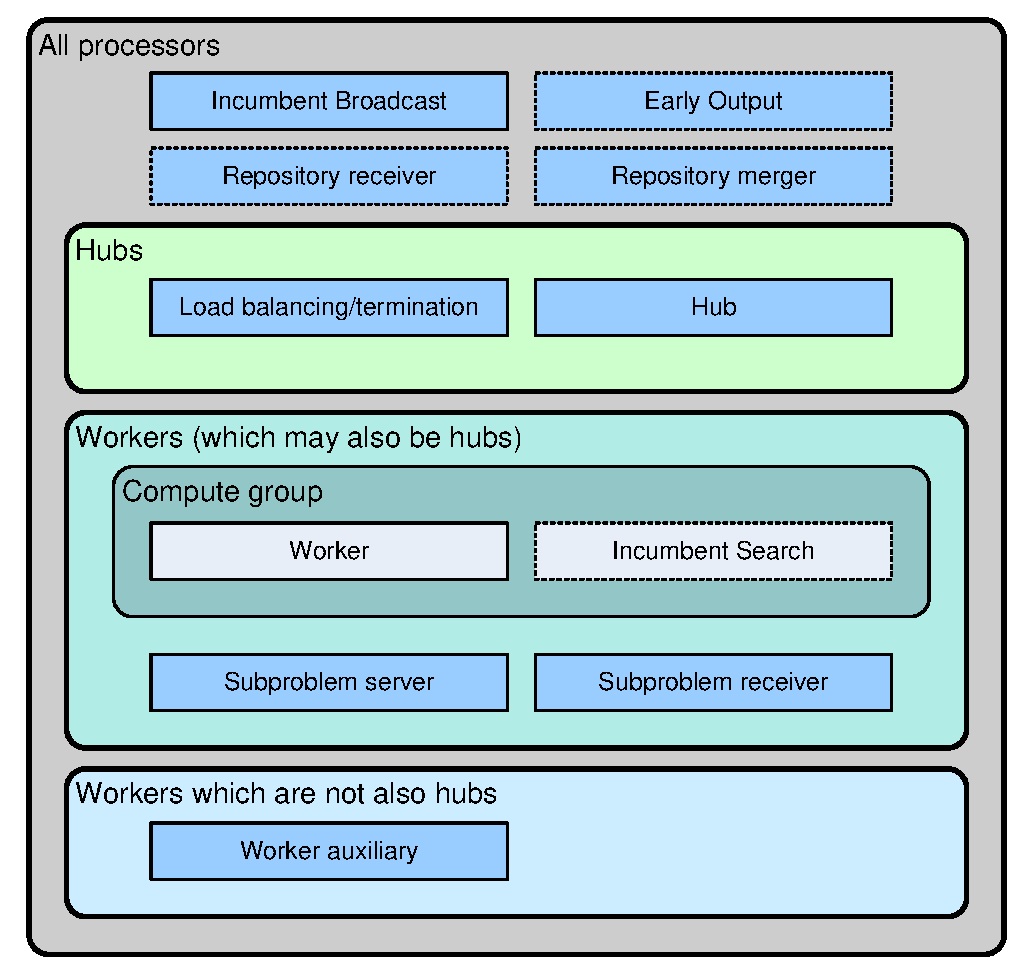
\includegraphics[width=0.7\textwidth]{threads-new}
\vspace{-0.2in}
\end{center}
\caption{PEBBL's standard threads.  A dashed outline
indicates that the thread may not exist in some cases.}
\label{fig:threads}
\end{figure}

Figure~\ref{fig:threads} depicts PEBBL's standard threads. You may add
additional threads of your own, but that is an advanced topic not
currently covered in this guide.  The standard threads are as follows:

\begin{description}

\item[Incumbent broadcast thread:] This message-triggered thread is
  active on all processors.  Its job is to make sure that all
  processors become aware, as soon as possible, of the objective value
  used to prune the search tree.  It implements a form of
  asynchronous broadcast using a tree with an adjustable branching
  factor.

\item[Early output thread:] This message-triggered thread is active on
  all processors if the parameter \texttt{earlyOutputMinutes} is
  positive; otherwise it is absent. This thread coordinates the
  process of writing solution files, making sure the file is written
  by a processor that is priviledged to do I/O (the MPI standard
  specifies that not all processors, and perhaps only one processor,
  must have file and console output capabilities).

\item[Repository receiver thread.]  This thread is active on all
  processors if PEBBL is enumerating multiple solutions.  It handles
  the receipt of most messages involved in coordinating the individual
  repository segments on each processor into a global asynchronous
  repository.

\item[Repository merger thread.]  This thread active is on all
  processors whenever the parameter \texttt{enumCount} is greater than
  1.  When \texttt{enumCount} is in use, certain messages required to
  maintain a global estimate of the cutoff solution may be sent on a
  time-delayed basis to limit peak message volumes; the repository
  merger thread handles this ``throttled'' message sending process.

\item[Hub thread:]  This thread is active on all hub processors, and
  responds to messages from workers; these messages contain
  acknowledgements of received subproblems, tokens for released
  subproblem, and worker load information.  Note that a hub
  processor's work distribution functions may also be activated in
  other situations besides receipt of one of these messages, via the
  \texttt{parallelBranching::activateHub()} method. 

\item[Load balancing/termination thread:] This thread is active on
  all hub processors, and manages termination detection.  It also
  controls checkpointing if \texttt{checkPointMinutes} is positive.  When
  there is more than one cluster, it also manages the balancing of
  workload between clusters.  It is generally message-triggered, but
  in multi-cluster situations it may also self-activate on some
  processors via the \texttt{ready()} predicate called by the scheduler.

\item[Worker thread:] This compute thread is active on all worker
  processors, and manages the processing of subproblems.

\item[Incumbent heuristic thread:] This optional compute thread may be
  active only on workers, and is controlled by the parameter
  \texttt{useIncumbentThread}.  Its purpose is to heuristically search
  for improved incumbent solutions.  Packaging this function into a
  compute thread allows PEBBL to directly control the fraction of CPU
  resources being dedicated to heuristic incumbent construction; the
  bias of this thread automatically adjusts based on the \emph{relative
  gap}, the relative difference between the incumbent value
  and the best known bound among active search tree nodes.  However,
  if the worker thread becomes idle (because it has no subproblems to
  process), the incumbent search thread will attempt to use all
  available CPU resources on the worker.  This behavior can be useful
  near the beginning of a run if the number of subproblems at the end of
  the ramp-up phase is less than the total number of worker
  processors: instead of being totally idle, worker
  processors attempt to heuristically find incumbents until their
  worker threads receive subproblems.

\item[Subproblem server thread:] This message-triggered thread is
  active on all worker processors.  It receives messages from the hub
  processors, and may in response send subproblems to other workers
  for processing.

\item[Subproblem receiver thread:]  This message-triggered thread is
  active on all worker processors, receiving subproblems for processing.

\item[Worker auxiliary thread:] This message-triggered thread is
  active on workers that are not also functioning as hubs.  The hubs
  send this thread various instructions, such as to write a
  checkpoint, check for termination, or terminate the search process.
  The worker auxiliary thread also periodially receives information
  relevant to the load balancing algorithms.

\end{description}



\section{Creating PEBBL Applications}

When using PEBBL, you should generally first create a serial PEBBL
application and debug it using whatever C++ development tools
you are most comfortable with.  Then you should extend it to a
parallel application using MPI.

\subsection{Compiling and linking your application}
In developing a new PEBBL application, you may either keep your source
files outside the \texttt{acro-pebbl} directory tree, or incorporate
them into the tree.  If you keep your files outside, you should
inspect the results of the PEBBL \texttt{make} command or the contents
of \texttt{acro-pebbl/test/build.out}, and use compatible commands to
compile and link your application source files.  In particular, your
compile commands' \texttt{\#include} path should contain the directory
\texttt{acro-pebbl/include}, and your link commands should include the
libraries \texttt{acro-pebbl/lib/libpebbl.a} and
\texttt{acro-pebbl/lib/libutilib.a}.  In standard unix/Linux
environments, for example, you could use the compiler/linker directives
\begin{codeblock}
-I\textrm{[\emph{path}}/\textrm{]}acro-pebbl/include
-L\textrm{[\emph{path}}/\textrm{]}acro-pebbl/lib -lpebbl -lutilib
\end{codeblock}
An alternative approach is to place your application source and header
files within the PEBBL directory tree and use PEBBL's own compilation
tools to compile your code.  The recommended location for both your
source and header files is \url{acro-pebbl/src/example/pebbl}.  To
incorporate your files into PEBBL's build process, you should proceed
as follows:
\begin{enumerate}
\item Modify the file \url{acro-pebbl/src/Makefile.am}
  to include your new source files in a pattern similar to those for
  the \texttt{knapsack} application.  
\item Incorporate any
  new header files you have created into the list contained in the
  file \url{acro-pebbl/src/headers/Makefile.am}.  
\item Rerun the configuration and compilation procedure of
  Section~\ref{sec:compile}.  The \texttt{configure} step, guided by
  your altered \texttt{Makefile.am} files, will incorporate your
  application into PEBBL's build process.
\end{enumerate}

\subsection{Defining a serial application}
\label{sec:serialMethods}
To create a basic serial PEBBL application, you need to:
\begin{itemize}
\item Define a class extending \texttt{branching}
\item Define a class extending \texttt{branchSub}
\item If necessary, create a class extending \texttt{solution}
\item Create a ``driver'' program that runs your algorithm.
\end{itemize}
You may concentrate your code for all these purposes in a single C++
file.  Conventionally, however, you would use a header (\texttt{.h} or
\texttt{.hpp}) file to define your new classes, one or more additional
C++ source files containing code to implement methods for those
classes, and a separate C++ source file containing the driver.

To load the basic definitions of \texttt{branching},
\texttt{branchSub}, and \texttt{solution} 
into the compiler, you should \texttt{\#include}
the file \texttt{<pebbl/branching.h>}.  Supposing your classes are
called \texttt{\emph{myBranching}} and \texttt{\emph{myBranchSub}},
and you are using a single header file, it should take the general
form shown in Figure~\ref{fig:code1}.

\begin{figure}[tbp]
\begin{center}
\fbox{
\begin{minipage}{0.96\textwidth}
\vspace{1ex}
\begin{codeblock}
\#include <pebbl/branching.h> \\
\\
using namespace pebbl; \\
\\
class \emph{myBranchSub};  // Forward declaration \\
\\
clas\=s \emph{myBranching} : virtual public branching \\
\{\\
\>friend class \emph{myBranchSub}; \\
\\
public:\\
\>$\quad\vdots$ \\
\>\textit{myBranching\textrm{ methods and data here}} \\
\>$\quad\vdots$ \\
\} \\
\\
class \emph{myBranchSub} : virtual public branchSub \\
\{\\
\>friend class \emph{myBranching}; \\
\\
protected:\\
\>// A pointer to the global branching object\\
\> \emph{myBranching}* globalPtr;\\
$\quad\vdots$ \\
public:\\
\>  // Return a pointer to the global branching object\\
\>  \emph{myBranching}* global() const \{ return globalPtr; \}\\
\\
\>  // Return a pointer to the base class of the global branching object \\
\>  branching* bGlobal() const \{ return global(); \}\\
\>$\quad\vdots$ \\
\>\textit{myBranchSub\textrm{ methods and data here}} \\
\>$\quad\vdots$ \\
\}
\end{codeblock}
\vspace{0.2ex}
\end{minipage}
}
\end{center}
\vspace{-2ex}
\caption{Standard code pattern for creating a serial PEBBL application.}
\label{fig:code1}
\end{figure}

We now describe how to construct these classes; in the course of this
description, you may also refer to the files \texttt{serialCore.h},
and \texttt{serialKnapsack.\{h,cpp\}}
%%
%% WEH TODO - INSERT SEMI_ASSIGNMENT PROBLEM
%%
%%, and \textbf{insert the semi-assignment example} 
%%
in the directory \url{acro-pebbl/packages/pebbl/src/example/pebbl}.

\subsubsection{Methods you should create ---
  \texttt{branching}-derived class}

In your \texttt{branching}-derived derived class, for example
\texttt{\emph{myBranching}}, you should define the following methods:

\boxheader{Constructor}
Classes derived from \texttt{branching} should have a constructor with
no arguments; the diamond inheritance pattern used by PEBBL means that
constructors with arguments are in general not advisable for 
\texttt{branching}- and \texttt{branchSub}-derived classes.  The
constructor should contain a call to
\texttt{branching::\linebreak[0]branchingInit($\cdots$)}. If you want
to maximize the objective function, you should supply
\texttt{branchingInit} an argument of \texttt{maximization}; if you
want to minimize, you can leave the argument list blank, or supply the
argument \texttt{minimization}.  Thus, one might have something like
\begin{codeblock}
\emph{myBranching}()  \\
\{ \\
~~~\=branchingInit(minimization); \\
\>~~$\vdots$ \\
\}; 
\end{codeblock}
The direction of minimization is stored in the data member
\texttt{branching::sense}.  The values \texttt{minimization} and
\texttt{maximization} are C++ \texttt{enum} values, equal to $+1$ and
$-1$, respectively.

\boxheader{Destructor} 
Naturally, you should also have a destructor for your
\texttt{branching}-derived class, for example:
\texttt{$\sim$\emph{myBranching}() \{ $\cdots$ \};}.

\method{branchSub* blankSub()}
You must provide a \texttt{blankSub()} method of return type
\texttt{branchSub*} that returns an empty subproblem specific to your
application.  To avoid circularity, the class declaration for
\texttt{\emph{myBranching}} should declare this method, but not
include its code, as in:
\begin{codeblock}
branchSub* blankSub();
\end{codeblock}
Once
\texttt{\emph{myBranching}} and
\texttt{\emph{myBranchSub}} are both declared, you should have the
actual code, for example:
\begin{codeblock}
bra\=nchSub* \emph{myBranching}::blankSub() \\
\{ \\
\>   \emph{myBranchSub}* newSP = new \emph{myBranchSub}; \\
\>    newSP->setGlobalInfo(this);\\
\>    return newSP; \\
\};
\end{codeblock}
Here, \texttt{\emph{myBranchSub}::setGlobalInfo} is a method that is
required to be a member of the subproblem class (see
Section~\ref{sec:bsubmethods} below), and
copies any necessary information from the 
\texttt{\emph{myBranching}} object into a \texttt{\emph{myBranchSub}}
object.  At a minimum, it should set the subproblem's
\texttt{globalPtr} member.  

\method{bool setupProblem(int\& argc,char**\& argv)}
This method is responsible for reading in any input data describing
the problem instance.  Its arguments \texttt{argc} and \texttt{argv}
are standard unix-style command line descriptors.  However, by the
time \texttt{setupProblem} is called, these arguments will be
``cleaned'' of any MPI-related information and parameter settings
recognized by PEBBL.  Typically, \texttt{setupProblem} should simply
read a problem description from the file whose name is pointed to 
by \texttt{argv[1]}.  The \texttt{setupProblem} method should return
\texttt{true} is problem setup was successful.

%% \method{serialPrintSolution(const char* header,const char*
%%   footer,std::ostream\& s)} 
%% Typically, the \texttt{branching}-derived class should have the
%% ability to store a single solution to the optimization problem.  The
%% \texttt{serialPrintSolution} method should print this solution to the
%% stream \texttt{s}, preceded by the \texttt{header}, and followed by
%% \texttt{footer}.  Strictly speaking, you do not have to implement this
%% method --- it has a default implementation of \texttt{\{~\}}.
%% However, it should be defined if you need PEBBL to print
%% out anything besides the \emph{value} of the solution.

\method{void reset(bool resetVB = true)} Perform any initializations
needed after \texttt{setupProblem} and before solving the actual
problem.  For some applications, the default implementation
\texttt{branching::reset} may suffice.  The optional argument
\texttt{resetVB} indicates whether virtual base classes should be
reset as well; it is present to allow one to avoid multiple redundant
initializations of such bases classes.  Typically, it can be ignored,
although there may be a minor performance penalty.  If you override the
\texttt{reset} method, make sure your implementation invokes
\texttt{branching::reset} in addition to any application-specific
initializations it performs.

\subsubsection{Methods you should create ---
  \texttt{branchSub}-derived class}
\label{sec:bsubmethods}

\boxheader{Constructor} 
As with the \texttt{branching}-derived class,
you should have an empty-argument constructor for your
\texttt{branchSub}-derived class, for example:
\begin{codeblock}
\emph{myBranchSub}() \{  $\cdots$ \}; \\
\end{codeblock}

\boxheader{Destructor} 
A destructor is naturally required, for example:
\begin{codeblock}
$\sim$\emph{myBranchSub}() \{ $\cdots$ \}; \\
\end{codeblock}

\method{branching* bGlobal() const}
This method is required for methods in \texttt{branchSub} to locate
the corresponding problem-wide information in the corresponding
\texttt{branching} object.  Presuming you have declared a data member
\texttt{\emph{myBranching}* globalPtr} as in Figure~\ref{fig:code1}, 
then Figure~\ref{fig:code1}'s definition should suffice:
\begin{codeblock}
branching* bGlobal() const \{ return global(); \};
\end{codeblock}
Your implementations of methods such as \texttt{boundComputation()}
will almost certainly require access to problem-wide but
application-specific information.  In the implementation above, this
may be obtained directly through \texttt{globalPtr} or slightly more
elegantly via
\begin{codeblock}
\emph{myBranching}* global() const \{ return globalPtr; \};
\end{codeblock}

\method{void setGlobalInfo(\emph{myBranching*} global\_)}
The purpose of this routine should be to ``bind'' a particular
subproblem object to the problem description embodied in the object
\texttt{*global\_}.  At a minimum, this requires setting
\texttt{globalPtr}.  For example:
\begin{codeblock}
voi\=d setGlobalInfo(\emph{myBranching*} global\_) \\
\{ \\
\> globalPtr = global\_; \\
\>\textrm{(Copy any other desired information from
  \texttt{*global\_} )}\\
\}
\end{codeblock}


\method{void setRootComputation()}
A call to this method indicates that a \texttt{\emph{myBranchSub}}
object should be made into a root subproblem.  Information on the
problem instance should be obtained, for example, via
\texttt{global()} or \texttt{globalPtr}.

\pagebreak[1]

\method{void boundComputation()} 
This method should attempt to bound the subproblem.  When the bound
computation is complete, it should execute \texttt{setState(bounded)}.
If the method exits without calling \texttt{setState(bounded)} to
declare the subproblem \texttt{bounded}, PEBBL will assume that the
bounding operation is incomplete: it will call
\texttt{boundComputation()} repeatedly (but perhaps not immediately) 
until the subproblem is
fathomed or declared \texttt{bounded}.  To indicate the value of the
bound, you set the \texttt{double} data member \texttt{bound};
you may update \texttt{bound} as many times as you like, and PEBBL
will use the information immediately, even before the
problem state becomes \texttt{bounded} --- for example, a sequence of calls
to \texttt{boundComputation()} may gradually improve the bound.
To indicate infeasibility of a subproblem, or that it cannot possibly
improve upon the current solution stored in
\texttt{bGlobal()->incumbentValue}, you may execute
\texttt{setState(dead)}. 


\method{bool candidateSolution()} PEBBL will only invoke this method
for subproblems in the \texttt{bounded} state.  Returning
\texttt{true} means that the just-computed bound is \emph{exact}: not
only is it a bound on all solutions in the region of the search space
corresponding to the subproblem, but that bound is also attained by at
least one feasible solution in that region.  Unless one is enumerating
multiple solutions, such a subproblem is considered a \emph{terminal}
node of the branch-and-bound tree, and will not be separated.  In
integer programming, for example, you would want
\texttt{candidateSolution()} to return \texttt{true} whenever the
linear programming relaxation produces a solution that has all integer
values.  Returning \texttt{true} also indicates to PEBBL that you have
computed a feasible solution to the overall optimization problem, as
opposed to just a bound.  PEBBL will most likely invoke
\texttt{extractSolution()} (see below) to retrieve this solution.


\method{solution* extractSolution()} PEBBL will only call this method
for \texttt{bounded} subproblems for which \texttt{candidateSolution}
has returned \texttt{true}.  The method should return a pointer to a
\texttt{solution}-derived object containing a solution corresponding
to the subproblem bound.  See Section~\ref{sec:solclassdetails} for
more information on \texttt{solution} objects.  Ownership of the
returned object is ceded to PEBBL.


\method{int splitComputation()} 
This method should attempt to separate the subproblem.  Similarly to
\texttt{boundComputation()}, it will be invoked repeatedly until it
calls \texttt{setState(separated)}.  The value returned is the number $k$
of child problems generated (simply $2$ for many applications).  The
number of children can vary between subproblems.
If you return without declaring the problem \texttt{separated}, PEBBL
will ignore the return value and invoke \texttt{splitComputation()}
again later.  In the course of separating the problem, you may update
\texttt{bound} at any time to reflect any further information gained
in the course of separation; PEBBL will use this
information immediately.  This routine may also execute
\texttt{setState(dead)}, in which case PEBBL will immediately prune
the subproblem.

If PEBBL is not in enumeration mode, it will call
\texttt{splitComputation()} only for nodes for which
\texttt{candidateSolution} has returned \texttt{false}.  On the other
hand, if PEBBL is enumerating multiple solutions, it is possible that
\texttt{splitComputation()} may be called for nodes for which
\texttt{candidateSolution} has returned \texttt{true}.  If you need
your application to be compatible with enumeration, it should be able
to handle this case of separating an otherwise ``terminal''
subproblem.  In some applications, such
nodes may require a completely different separation technique than
other nodes, and possibly a different number of children.  Ideally,
when separating a subproblem $P$ for which \texttt{candidateSolution}
has returned \texttt{true}, you should create one or more children
corresponding to search-space regions which are disjoint and contain
all solutions corresponding to $P$ \emph{except} the one just returned
by $P\!$\texttt{.extractSolution()}.  This latter solution will already
be known to PEBBL and need not be examined again.  If a node is
``truly terminal'' in that it corresponds to a subset of the search
space containing only a single distinct feasible solution, then
\texttt{splitComputation()} should call \texttt{setState(dead)} and
return $0$.

\method{branchSub* makeChild(int whichChild)} 
This method should create a child problem and return a pointer to it.  
The argument
\texttt{whichChild} may take any value between $0$ and $k-1$, where $k$
was the value returned by \texttt{splitComputation()} for this
subproblem.  
A value of $0$ indicates you should create the first child, a
value of $1$ indicates you should create the second child, and so
forth.  

When you create a child problem, you should make sure that its
\texttt{globalPtr} is set as in the parent problem, and all local
data are initialized correctly.  In order for PEBBL to correctly track
subproblem depth and counts of created subproblems, it is also necessary to
correctly set up various data members of the \texttt{branchSub} class.  PEBBL
provides a method called \texttt{branchSubAsChildOf} to perform this
operation.  Specifically, the child problem should invoke
\texttt{branchSubAsChildOf(parent)} soon after it is created, where
\texttt{parent} is a pointer to the parent subproblem.  Alternatively, the parent
subproblem may call
\begin{codeblock}
\emph{child}->branchSubAsChildOf(this);
\end{codeblock}
where \emph{\texttt{child}} is a pointer to the child subproblem just created.


%% \method{void updateIncumbent()}
%% This method should set the state of the \texttt{branching}-derived
%% class --- \emph{e.g. \texttt{myBranching}} --- to reflect a feasible
%% problem solution correspondig to this 
%% subproblem.  PEBBL will typically call this method
%% after \texttt{candidateSolution()} returns \texttt{true}.  A typical
%% implementation will look like:
%% \begin{codeblock}
%% voi\=d \emph{myBranchSub}::updateIncumbent() \\
%% \{\\
%% \>bGlobal()->incumbentValue = bound;  // Set the incumbent value \\
%% \>\textrm{(Copy the solution itself to \texttt{*global()})} \\
%% \>bGlobal()->signalIncumbent(); \\
%% \}
%% \end{codeblock}
%% Once the solution has been copied to a \texttt{branching}-derived
%% class, it can be written by the \texttt{serialPrintSolution($\cdots$)}
%% method.  The call to \texttt{signalIncumbent()} tells PEBBL that
%% the subproblem pool should be pruned.  Once the application is ported
%% to the parallel layer, \texttt{signalIncumbent()} will also initiate
%% interprocessor communication to broadcast the new incumbent value.


\subsubsection{The \texttt{solution} class and related methods}
\label{sec:solclassdetails}
PEBBL manipulates feasible problem solutions via objects whose type is
derived from \texttt{solution}.  For example, the
\texttt{extractSolution()} method should return a \texttt{solution*},
as should the \texttt{initialGuess} method; see
Section~\ref{sec:seradd} below.  The \texttt{solution} class itself
contains (among others) the following members:
\begin{description}
\item{\texttt{double value}}: the solution's objective value.
\item{\texttt{int serial}}: a serial number (assigned automatically by
  PEBBL).
\item{\texttt{size\_type hashValue}}: a value for use in hash tables
\end{description}
It is possible to represent solutions via the \texttt{solution} base
class; however, such a representation will essentially contain only
the solution's objective value, and no other information.  
To construct such an object, use the
constructor \texttt{solution(branching*)}, and then set the
\texttt{value} of the resulting object.  For example, for the code in the
\texttt{\emph{myBranchSub}} class of Figure~\ref{fig:code1}, one would
use
\begin{codeblock}
s = new solution(global()); \\
s.value = \emph{objective value};
\end{codeblock}
Far more likely, however, you will want a true solution representation
that contains more information than just the objective value.  In this
case, you should use another class derived from \texttt{solution}.  Here,
there are two choices: use the template class
\texttt{arraySolution<\emph{T}>}, or derive your own \texttt{solution}-based
class.

Note that each instance of the \texttt{solution} class contains its
own \texttt{sense} member which must be set to \texttt{maximization}
or \texttt{minimization} consistently with \texttt{branching}-derived
object describing the problem instance (for example,
\texttt{\emph{myBranching}}).  Typically, this is handled by passing a
\texttt{branching*} pointer to the \texttt{solution} constructor.

Starting with PEBBL 1.6, the \texttt{solution} class includes a reference
counter, and its destructor will throw an exception if activated when this
counter is nonzero.  One should not directly invoke the destructors of
\texttt{solution}-derived objects by using the
\texttt{delete} operator, but instead use the \texttt{dispose()} method of the
\texttt{solution} class.  This method decrements the reference counter and then
call the destructor if the counter is zero.  The reference counter may also be
incremented or decremented by the \texttt{incrementRefs()} and
\texttt{decrementRefs()} methods, respectively.  If a
\texttt{solution}-derived object is allocated on the stack by direct
declaration, rather than by using the \texttt{new} operator, one should call
its \texttt{decrementRefs()} method before it passes out of scope; otherwise
its destructor will trigger an exception.

The template \texttt{arraySolution<\emph{T}>} is a ready-made PEBBL-supplied
class that represents a solution as a one-dimensional array (that is,
a vector) of some type \texttt{\emph{T}} which may be implicitly converted to
a \texttt{double} without loss of information.  To create such a
solution object, invoke a constructor (supplied by PEBBL) of the form
\texttt{arraySolution<\emph{T}>($z$,$v$,$b$,$t$,$\nu$)}, where:
\begin{quote}
\begin{description}
\item[$z$] denotes the objective value of the solution 
\item[$v$] is either a UTILIB array object of type
  \texttt{BasicArray<\emph{T}>}, an STL vector of type 
  \texttt{vector<\emph{T}>}, or
  some object derived from either of those possibilities (for example,
  the UTILIB \texttt{IntVector} type derives from
  \texttt{BasicArray<int>}, and may thus be used to create an
  \texttt{arraySolution<int>}).  This information is copied into the
  new \texttt{arraySolution} object.
\item[$b$] is a pointer
  to the \texttt{branching}-derived object describing the 
  problem instance; within the class \texttt{\emph{myBranchSub}} of
  Figure~\ref{fig:code1}, you would set $b =
  \text{\texttt{global()}}$, and within the
  \texttt{\emph{myBranching}} of Figure~\ref{fig:code1}, you would set
  $b = \text{\texttt{this}}$.  One function of this argument is to
  make sure that the maximization/minimization \texttt{sense} of the
  \texttt{arraySolution} is set correctly.
\item[$t$] is optional, and is simply a \texttt{const char*} pointing to a
  description of the type of solution, for example, \texttt{"Vector
    of integers"}. 
\item[$\nu$] is also optional, and is a pointer to a
  \texttt{BasicArray<CharString>} object containing names of the
  decision variables.  It should be at least as long as $v$.  These
  names are used when printing the solution contents.  
\end{description}
\end{quote}
For descriptions of the types \texttt{BasicArray} and
\texttt{CharString}, see the UTILIB documentation.

If \texttt{arraySolution} does not apply to your problem, is
inconvenient, or will be inefficient, you should derive your own
class of objects from \texttt{solution}, as in:
\begin{codeblock}
class \emph{mySolution} : virtual public solution \{ $\cdots$ \}
$\;.$
\end{codeblock}
You may use more than one kind of solution class in a single
application.  

To facilitate hashing and comparison, solutions normally
have a ``sequence representation'', as described in
Section~\ref{sec:solclass}.  This representation is essentially a
one-dimensonal array of \texttt{double}s, although it need not be (and
probably should not be) explicitly stored.  By default, PEBBL uses
this sequence representation to compute a solution's
\texttt{hashValue} and to compare two solutions to detect duplicates.
The solutions are considered duplicates if and only if their sequence
representations are identical in both length and contents.

In addition to application-specific data members describing a
solution, a customized solution class like \texttt{\emph{mySolution}}
should typically define the following \texttt{virtual} methods:

\vspace{2ex}

\boxheader{Constructor}
To create the underlying \texttt{solution} object, your solution constructor
should invoke the \texttt{solution(branching*)} constructor.  It should also
set the \texttt{value} member to reflect the solution's objective
value.  For the \texttt{\emph{myBranching}},
\texttt{\emph{myBranchSub}}, classes, for example, the standard
constructor pattern would be
\begin{codeblock}
\emph{mySolution}(\=\emph{myBranching}* global\_, \\
                  \>\textrm{[}, \textrm{\emph{other arguments}]}) : \\
~~~solution(global\_), \\
~~~$\cdots$ \\
\{ \\
~~~value = $\cdots$; \\
~~~\textrm{[\emph{Set internal representation of solution}]} \\
\}
\end{codeblock}
Note that in the invocation of \texttt{solution(global\_)}, the
\texttt{\emph{myBranching*}} pointer \texttt{global\_} is
automatically cast to a base class pointer of type
\texttt{branching*}. 

\boxheader{Destructor}
A destructor should be provided.  However, as noted above, it should not be
invoked directly through \texttt{delete}, but through the \texttt{solution}
class' \texttt{dispose()} method.

\method{const char* typeDescription() const} Returns a \texttt{const
  char*} describing the type of solution, for example
\texttt{"Knapsack solution"}.

\method{virtual void printContents(std::ostream\& s)} Write the
solution contents (for example the decision variable values) to the stream
\texttt{s}.  You do not need to write the objective value; it is
printed by another method.  The default implementation is a stub.

\method{virtual size\_type sequenceLength()}  Return the number of
elements in the sequence representation of the solution.  

\method{virtual double sequenceData()} Return the next element of the
sequence representation.

\vspace{2ex}

The following method is related to \texttt{sequenceData()} and
\texttt{sequenceLength()}, but may not have to be overridden:

\vspace{2ex}

\method{virtual void sequenceReset()} Cause the next call to
\texttt{sequenceData()} to return the first element in the sequence.
The default implementation is simply to set the data member
\texttt{sequenceCursor} (built into the \texttt{solution} class) to
zero.

\vspace{2ex}

Note that PEBBL will call \texttt{sequenceData()} at most
\texttt{sequenceLength()} times between calls to
\texttt{sequenceReset()}.  Typically, the default implementation of
\texttt{sequenceReset()} will suffice, and each call to
\texttt{sequenceData()} should return the
$\text{\texttt{sequenceCursor}}^\text{th}$ element of the sequence and
then increment \texttt{sequenceCursor}.

It is not absolutely necessary that a solution have a sequence
representation, and thus not absolutely required that you define
\texttt{sequenceLength()} and \texttt{sequenceData()}.  If you do not
define those methods, however, you must define two other methods:

\vspace{2ex}

\method{size\_type computeHashValue()} Return the hash value of the
solution.

\method{bool duplicateOf(solution\& other)} Return \texttt{true} if
\texttt{other} is an identical solution, and otherwise
\texttt{false}. 

\vspace{2ex}

Normally, it is recommended that you simply retain the default
implementations of these methods, and define application-specific
versions of \texttt{sequenceLength()}, \texttt{sequenceData()}, and
possibly \texttt{sequenceReset()}.  The default implementations of
\texttt{computeHashValue()} and \texttt{duplicateOf} are based on the
sequence representation.  Even if you have defined a sequence
representation, you may elect to override \texttt{computeHashValue()}
and/or \texttt{duplicateOf} to improve efficiency.


\subsubsection{The \texttt{foundSolution} method}
So far, the only means we have discussed for providing solutions to
PEBBL is the method \texttt{extractSolution} (see
Section~\ref{sec:bsubmethods}), which PEBBL calls between
\texttt{boundComputation} and \texttt{splitComputation} for
subproblems whose bounds are known to be exact.  Many branch-and-bound
algorithms encounter feasible solutions at other points in the search
process.  When this occurs, you may call the method
\texttt{branching::foundSolution(solution* sol)}, where \texttt{sol}
is a pointer to a \texttt{solution}-derived object.  You need not
first ascertain whether \texttt{*sol} is a better solution than the
incumbent, or, when enumerating multiple solutions, whether it is
eligible to enter the repository.  PEBBL will determine whether the
solution is useful, and otherwise delete it.  Note that calling
\texttt{foundSolution(sol)} cedes memory ownership of one reference to
\texttt{*sol} to PEBBL.  If the caller would like to continue using
\texttt{*sol} after calling \texttt{foundSolution(sol)}, the following apply:
\begin{itemize}
\item The caller should invoke \texttt{sol->incrementRefs()} before calling 
\texttt{foundSolution(sol)}
\item The caller should not alter the contents of \texttt{*sol}
solution after calling \texttt{foundSolution(sol)}, since doing so could cause
internal errors or unpredictable behavior in PEBBL
\item Once it no longer needs \texttt{*sol}, the caller should invoke
\texttt{sol->dispose()}.
\end{itemize}
If the caller does not have further need of \texttt{*sol} after calling
\texttt{foundSolution(sol)}, no action is necessary.

It is safe to call \texttt{foundSolution} at any point within the
branch-and-bound tree exploration, for example, from within the
methods \texttt{boundComputation}, \texttt{splitComputation} and
\texttt{makeChild}.  For example, from the \texttt{boundComputation}
method of the hypothetical \texttt{\emph{myBranchSub}} class, you
could invoke \texttt{foundSolution} via
\texttt{global()->foundSolution(sol)}.  You should not call
\texttt{foundSolution} at points before the branch-and-bound search
has begun (for example, in the \texttt{setupProblem} method or the
\texttt{preprocess} method described immediately below), or after the
search has concluded.  To provide a rough initial solution before the
tree exploration process has started, use the \texttt{initialGuess}
method described immediately below.


\subsubsection{Selected additional methods}
\label{sec:seradd}
We now present an inexhaustive list of additional methods that you may
wish to override for particular applications.

\method{void branching::preprocess()}
This method is intended for ``preprocessing'' of the problem prior to
commencing the branch-and-bound search; the default implementation is
an empty stub.  In principle, its functions
could be combined with \texttt{setupProblem($\cdots$)}, but it is
provided for clarity and to ease migration to the parallel layer.
%% Note that once you migrate your application
%% to the parallel layer, \texttt{preprocess()} is called \emph{after}
%% the problem instance is broadcast to all processors, and could
%% potentially be parallelized.

\method{solution* branching::initialGuess()} PEBBL calls this method
between preprocessing and the start of the branch and bound search.
Its intention is allow computation of a ``quick and dirty'' initial
guess at the solution.  In a knapsack problem, for example, this
routine could run a simple greedy heuristic.  Your implementation need
not be guaranteed to find a usable solution; if it does not, it should
just return a \texttt{NULL} pointer.  The default implementation is a
stub that simply returns \texttt{NULL}.

\method{bool branching::haveIncumbentHeuristic()} 
The default implementation of this method just returns \texttt{false}.
You should change it to return \texttt{true} if your application has a
way of trying to obtain a feasible solution from a non-terminal
\texttt{bounded} subproblem.  

\method{void branchSub::incumbentHeuristic()} 
This method applies only to the serial layer, and PEBBL will only call
it directly if the method \texttt{haveIncumbentHeuristic()} returns
\texttt{true}.  PEBBL calls it at two points, once a solution has
become \texttt{bounded}, and once it has become \texttt{separated}. 
The intention is to allow the heuristic calculation of feasible
solutions.  Whenever your implementation finds a feasible solution, it
should communicate it to PEBBL by calling \texttt{foundSolution}.  The
default implementation is a stub.

You may wish to check the subproblem state at the beginning of your
implementation of \texttt{incumbentHeuristic}.  For example, if you
wish your heuristic to be invoked only when subproblems become
\texttt{bounded}, and not when then become \texttt{separated}, you
could begin your implementation with
\begin{codeblock}
if (state != bounded) return;
\end{codeblock}
If you wish to construct heuristic solutions at other points besides
when subproblems become \texttt{bounded} or \texttt{separated}, you
can create your own heuristic method and invoke it at other times,
having it call \texttt{foundSolution} to send new solutions to PEBBL.

Note that the parallel layer treats incumbent heuristics somewhat
differently, and parallel-layer runs will not explicitly call
\texttt{incumbentHeuristic}; see Section~\ref{sec:parMethods} below.
 
\method{void branchSub::makeCurrentEffect()} PEBBL has the notion of a
``current subproblem'' -- the one presently being bounded or
separated.  The method \texttt{makeCurrentEffect()} provides a
``hook'' that is called whenever a subproblem is made ``current''.  In
a branch-and-cut algorithm, for example, this method could load the
subproblem's cuts into the linear programming solver.  Its default
implementation is a stub.

\method{void branchSub::noLongerCurrentEffect()}
PEBBL calls this ``hook'' whenever a subproblem ceases to be
``current''.  Again, its default implemetation is a stub.

\method{bool branchSub::forceStayCurrent()}
PEBL calls this method when it is considering replacing the current
subproblem with a different one.  Returning \texttt{true} indicates
that the current subproblem should be kept current if at all possible.
The default implementation always returns \texttt{false}, meaning that
PEBBL is free to ``unload'' the current subproblem, and replace it
with a different one.

\method{bool branching::checkParameters()} PEBBL calls this method to
make sure that its runtime parameters are set correctly and
consistently.  You may override this method to perform additional
checks specific to your application, and then call
\texttt{branching::checkParameters()} to make sure PEBBL's internal
checks are invoked.  You are most likely to need this routine if you
have defined your own application-specific runtime parameters; see the
section immediately below.

\subsubsection{Creating your own parameters}
\label{sec:ownparams} 
In addition to PEBBL's existing parameters, you may create your own
command-line parameters.  The simplest place to do so is in the
constructor of your \texttt{branching}-derived class.  Alternately,
you can define a underlying base class to hold your parameters: you
could create a class \texttt{\emph{myParams}} to hold your parameters,
and then derive \texttt{\emph{myBranching}} from both
\texttt{branching} and \texttt{\emph{myParams}}.  Parameter creation
statements should usually reside in constructors and have the general
form
% The following null command stops sublime text from  miscoloring 
% the rest of the file
\newcommand{\nothing}{}  
\begin{codeblock}
create\_categorized\_parameter(\="\textrm{\emph{commandLineName}}",\\
\>\textrm{\emph{internalName}},\\
\>"\nothing<\textrm{\emph{datatype}}>",\\
\>"\textrm{\emph{defaultValue}}",\\
\>"\textrm{\emph{text description}}",\\
\>"\textrm{\emph{category}}"\textrm{[},\textrm{]}\\
\>\textrm{[\emph{error check object}]})
\end{codeblock}
Here,
\begin{description}
\item[\textmd{\emph{commandLineName}}] is the name to be recognized on
  the command line.  For example, \texttt{fooBar} will cause the
  option \texttt{--fooBar=\textrm{\emph{value}}} to be recognized on the
  command line.  
\item[\textmd{\emph{internalName}}] is a reference to a class data
  member in which to store the value of the parameter; usually,
  \emph{internalName} and \emph{commandLineName} should be identical
  for clarity.
\item[\textmd{\emph{datatype}}] is the C++ datatype of
  \emph{internalName}.  Common choices are \texttt{bool},
  \texttt{int}, \texttt{double}, and \texttt{string}.
\item[\textmd{\emph{defaultValue}}] is a text representation of 
  the default value for the
  parameter.  It should match the initial value stored in the data
  member \emph{internalName}.  Note that the specification of
  \emph{defaultValue} does not automatically initialize the value of
  \emph{internalName}; its initial value should be set by the class
  constructor and \texttt{reset} methods.
\item[\textmd{\emph{text description}}] is a parameter description
  printed in response to \texttt{--help}.  For descriptions longer
  than one line, embed newline-tab character sequences
  (``\texttt{$\backslash$n$\backslash$t}'') in this text.
\item[\textmd{\emph{category}}] The category header to be used when
  printing the parameter description in response to \texttt{--help}.
  You may invent new categories.
\item[\textmd{\emph{error check object}}] is optional and 
  specifies simple constraints
  on the value of the parameter.  For example,
  \begin{codeblock}
  ParameterNonnegative<int>()
  \end{codeblock}
  specifies that an integer parameter must be nonnegative, while
  \begin{codeblock}
  ParameterBounds<double>(0.0,1.0)
  \end{codeblock}
  specifies that a \texttt{double}-datatype parameter must have values
  between 0 and 1, inclusive.  Other common forms for error-check objects are
  \begin{codeblock}
  ~~~~\=ParameterLowerBound<\textit{datatype}>(\textit{minimum
      value}) \\
  \textrm{or}\>
  ParameterUpperBound<\textit{datatype}>(\textit{maximum
      value})
  \end{codeblock}
  \noindent For more details, refer to the UTILIB \texttt{Parameter}
  and related class documentation.
\end{description}

For error checks that are more elaborate, or involve interactions
between multiple parameters, you may specify parameter error checks by
overloading the \texttt{checkParameters} boolean method in the
\texttt{branching} class, for example with
\texttt{\textit{myBranching}::checkParameters}; if this routine
detects an error, it should print a diagnostic message and return
\texttt{false}.  If it does not, it should execute \texttt{return
  branching::checkParameters()} to invoke the standard checks on
PEBBL's built-in parameters.

Note that for parameters of type \texttt{bool}, you may omit
\texttt{=}\emph{value} on the command line, in which case the value is
set to \texttt{true}.  That is, \texttt{--fooBar} is
equivalent to \texttt{--fooBar=true}


\subsubsection{Serial main programs: drivers}
\label{sec:serialdriver}
PEBBL is structured as a callable library, and can thus be
incorporated directly into other C++ applications.  If you want your
PEBBL application to function as a simple ``solver'' executable that
simply reads in a problem instance data file and solves it, you need
to create a ``driver'' main program.  A simple template function called
\texttt{driver} is available for this purpose.  Using this
template, you can construct the driver for the hypothetical example
application \texttt{\emph{myBranching}} as follows:
\begin{codeblock}
\textrm{\emph{Header file}} \#include\textrm{\emph{s, including}} 
\emph{myBranching} \textrm{\emph{class and}} <pebbl/branching.h> \\
\\
int \=main(int argc, char** argv)\\
\{\\
  \> return driver<\emph{myBranching}>(argc,argv);\\
\}
\end{codeblock}
Invoking \texttt{driver<\emph{myBranching}>(argc,argv)} 
is equivalent to the code shown in Figure~\ref{fig:serialdriver}.
Note that the main PEBBL header file \texttt{<pebbl/branching.h>}
automatically includes the necessary UTILIB header files to define the
method \texttt{InitializeTiming()}.
\begin{figure}[tbp]
\begin{center}
\fbox{
\begin{minipage}{0.65\textwidth}
\vspace{1ex}
\begin{codeblock}
InitializeTiming(); \\
  \emph{myBranching} instance; \\
  boo\=l f\=lag = instance.setup(argc,argv); \\
  if (flag) \\
\>    \{ \\
\>\>      instance.reset(); \\
\>\>      instance.solve(); \\
\>    \}\\
  return !flag;
\end{codeblock}
\vspace{1ex}
\end{minipage}
}
\end{center}
\vspace{-2ex}
\caption{Code equivalent to the serial
  \texttt{driver<\emph{myBranching}>(argc,argv)} template.}
\label{fig:serialdriver}
\end{figure}
Note also that \texttt{setup($\cdots$)}, \texttt{reset()}, and
\texttt{solve()} are all methods of the \texttt{branching} class that
you typically do not override.  Calling \texttt{setup(argc,argv)}
parses the command line, extracting and processing all command line
arguments recognizable as PEBBL parameters, including any 
application-specific parameters created as described in 
Section~\ref{sec:ownparams}.  It then calls your
implementation of \texttt{setupProblem}, with \texttt{argc} and
\texttt{argv} adjusted so that parameter-setting arguments are
removed; \texttt{setup}'s returning \texttt{true} indicates both that
all command line parameters were processed correctly, and that your
\texttt{setupProblem} implementation returned \texttt{true},
indicating it was successful.  The method \texttt{solve()} invokes the
branch-and-bound search engine, and prints subproblem count and timing
statistics upon termination.  It also uses your
\texttt{solution}-derived class' \texttt{printContents} implementation
to write the final solution(s) to a file whose name is derived from
the first command line argument not recognizable as a parameter
setting, typically by appending \texttt{sol.txt}; if no such parameter
can be found, the file is called \texttt{sol.txt}).  If you instead
wish to specify your own choice for the solution file, use the
\texttt{--output=}\emph{filename} command-line option.  Here,
\emph{filename} may contain path information, and thus need not be in
the current directory.

The \texttt{setup} method manages parsing of the command line
including option specifications and a problem instance data file name.
Supposing your driver were called \texttt{\emph{myDriver}}, the
command line \texttt{\emph{myDriver} \emph{datafile}} 
would call \texttt{\emph{myBranching}::setupProblem(argc,argv)} with
\texttt{argv[1]} containing the null-terminated string
\texttt{\emph{datafile}} --- with a typical implementation of
\texttt{setupProblem}, this would cause your application to read in
the problem instance description in \texttt{\emph{datafile}}.
In parsing the command line, \texttt{setup} will also recognize all PEBBL
command-line parameters (see Section~\ref{sec:param} for a partial
catalog) along with any parameters defined for
\texttt{\emph{myBranching}}, as described in
Section~\ref{sec:ownparams}.  For example, in the command line
\begin{codeblock}
\emph{myDriver} --relTolerance=0.05 --earlyOutputMinutes=2 \emph{datafile}
\end{codeblock}
the PEBBL parameters \texttt{relTolerance} and
\texttt{earlyOutputMinutes} would be set to $0.05$ and $2$,
respectively.  In this example,
\texttt{\emph{myBranching}::setupProblem(argc,argv)} would still be
called with \texttt{argv[1]} containing the null-terminated string
\texttt{\emph{datafile}}, presumably reading the problem instance in
\texttt{\emph{datafile}}. 
The \texttt{setup} method also automatically recognizes several
special command-line arguments:
\begin{description}
\item[\texttt{--help}] Causes \texttt{setup} to print a usage line
followed by a description of all available parameters, and then return
\texttt{false} (so that the driver above would not attempt to solve a
problem).  If you want to control the form of the usage line, override
the method \texttt{void branching::write\_usage\_info(char*
  progName,std::ostream\& os)}.  When PEBBL calls this method, the
argument \texttt{progName} is set equal to \texttt{argv[0]}.
\item[\texttt{--version}] must be the first argument if present.  It
  causes \texttt{setup} to print the value of the \texttt{static}
  \texttt{std::string} data member \texttt{branching::version\_info} and return
  \texttt{false} (so that the driver above would then immediately
  exit).  You may alter the contents of \texttt{version\_info}, for
  example, in the constructor for your \texttt{branching}-derived
  class.
\item[\texttt{--param-file=}\textmd{\emph{file}}] allows multiple parameter
  settings to be read from the file \emph{file} --- see the UTILIB
  Parameter class documentation for a description of the file format.
\end{description}

The \texttt{reset()} method invoked by the driver template performs
all necessary initializations prior to the solution process, which is
performed by \texttt{solve()}.  The \texttt{solve()} method in turn
invokes several lower-level methods, principally:
\begin{description}
\item{\texttt{search()}} to perform the actual branch-and-bound
  search.  
\item{\texttt{printAllStatistics()}} to print information about the
  number of search nodes and run time.
\item{\texttt{solutionToFile()}} to write the solution file.
\end{description}

\subsubsection{``Quiet'' operation}
If PEBBL is embedded within another application, it may be desirable to
have it run ``quietly'', without any configuration, status, or
performance-statistics printouts.  In this case, you should use the
\texttt{search()} routine instead of \texttt{solve()} and make sure
that solution status printouts are disabled by setting both
\texttt{branching::statusPrintCount} and \texttt{statusPrintSeconds}
to zero (see Section~\ref{sec:outputparams} for discussion of the
corresponding runtime parameters).

\subsubsection{Retrieving solutions to C++ code}
\label{sec:serialgetsol}
Note that PEBBL applications can be invoked in ways other than the
simple driver above; for example, they could be embedded in more
complicated C++ programs, in which case you would probably use the
\texttt{search()} method to perform the branch-and-bound search, and
avoid command-line-oriented methods like \texttt{driver},
\texttt{setupProblem}, and \texttt{solve()}.  

Various approaches are available to retrieve solutions computed by
running the \texttt{search()} method; note that all the methods described in
this subsection are members of the \texttt{branching} class.  If you
are not enumerating multiple solutions, you should simply use the method
\texttt{getSolution()}, which returns a \texttt{solution*} pointer to
the incumbent solution.  This method returns \texttt{NULL} if no
solution was found.  Within your application, the \texttt{solution*}
pointer returned by \texttt{getSolution()} will most likely need to be
cast ``up'' the inheritance hierarchy so that its contents may be
accessed, preferably using the C++ \texttt{dynamic\_cast} operator.

For retrieving multiple solutions from a run enumerating multiple
solutions, the simplest technique is to define an object
\texttt{\emph{solArray}} of type \texttt{BasicArray<solution*>} and
then call the method \texttt{getAllSolutions(\emph{solArray})}.  This
method will redimension \texttt{\emph{solArray}} to the size of the
repository and fill it with \texttt{solution*} pointers to the
repository members, in objective-value order, starting with the best
value.

For compatibility with the parallel layer, a second, iterator-like
technique is also possible.  In this approach, one first calls
\texttt{startRepositoryScan()}, which returns the size $n$ of the
repository.  One may then call \texttt{nextRepositoryMember()} up to
$n$ times: each time, it will return a different member of the
repository.  Again, solutions are returned in objective value order,
starting with the best values.

For any solution pointer \emph{\texttt{sol}} returned by \texttt{getSolution},
\texttt{getAllSolutions}, or \texttt{next\-Repos\-itory\-Member}, the application
should call \texttt{\emph{sol}->dispose()} when it no longer needs the
corresponding solution object.  As discussed in
Section~\ref{sec:solclassdetails}, one should never directly use
\texttt{delete} on \texttt{solution}-derived objects, because they are
reference-counted.

\subsubsection{Debugging outputs}
In the process of debugging a PEBBL application, it may be necessary
to print diagnostic outputs.  Through the companion UTILIB package
that it automatically includes, PEBBL provides special mechanisms for
such output.  The most frequently used is the \texttt{DEBUGPR} macro,
which takes the form
\begin{codeblock}
DEBUGPR(\textit{level},\textit{action});
\end{codeblock}
Inside a class derived from \texttt{branching}, such a statement
indicates that the code given by \texttt{\textit{action}} be executed
if the PEBBL debug output level specified by the run-time parameter
\texttt{debug} in Section~\ref{sec:debugparams} has a value of
\texttt{\textit{level}} or higher.  Typically,
\texttt{\textit{action}} should involve writing text to the
specialized stream \texttt{ucout}.  For example, the statement
\begin{codeblock}
DEBUGPR(10,ucout << "Value of n is " << n << endl);
\end{codeblock}
will print the value of the variable \texttt{n} whenever the debug output
level is at 10 or higher.  While it makes not difference in the serial
layer, using the special stream \texttt{ucout} is preferable to using
the standard stream \texttt{cout} because \texttt{ucout} has special
features that make it more convenient in a parallel setting.  In
particular, when used in parallel, each line of text sent to
\texttt{ucout} will be prefixed by a tag indicating which processor
wrote the information.

A slightly different form of debug printing is used in subproblem
classes derived from \texttt{branchSub}, as opposed to problem classes
derived from \texttt{branching}.  In this setting, the diagnostic
output above would instead be expressed as
\begin{codeblock}
DEBUGPRX(10,global(),ucout << "Value of n is " << n << endl);
\end{codeblock}
The reason for this difference is that, for efficiency reasons,
\texttt{branchSub} does not derive from the same UTILIB
\texttt{CommonIO} utility class that \texttt{branching} does.  

The \texttt{CommonIO} class from UTILIB makes several other variations
on the \texttt{DEBUGPR} available for specialized situations.  Consult
the UTILIB documentation for more information.

An advantage of using the \texttt{DEBUGPR} and related facilities
instead of \emph{ad hoc} print statements is that the diagnostic
output may be left in the code indefinitely and triggered whenever
needed by using the \texttt{debug} runtime parameter.  For example,
running a PEBBL application with the command-line option
\texttt{--debug=10} would set the debugging level to 10.  

\subsection{Defining a parallel application}
\label{sec:parMethods}
Now suppose that your serial layer applications runs acceptably, and
you wish to parallelize it.  If you want to use parallelism, be sure
that you have configured PEBBL with MPI; see Section~\ref{sec:compiling}, and
especially Section~\ref{sec:configoptions}.  In particular, you should
run \texttt{configure} with an option such as
\texttt{--with-mpi-compilers=yes} or
\texttt{--with-mpi-compilers=}\emph{pathname}.

When Acro is compiled with MPI, the preprocessor symbol
\texttt{ACRO\_HAVE\_MPI} is defined; otherwise it is not defined.
When \texttt{ACRO\_HAVE\_MPI} is undefined, only the serial portions
of PEBBL are compiled; the parallel portions are omitted or become
stubs.  You may wish to follow this same pattern within your own
application source code.

Figure~\ref{fig:code2} outlines the
recommended inheritance and pointer pattern for creating parallel
layer classes from a serial application.  Here, the serial layer
classes are \texttt{\emph{myBranching}} and
\texttt{\emph{myBranchSub}}, and the corresponding 
respective parallel layer classes
are \texttt{\emph{myParBranching}} and \texttt{\emph{myParSub}}.  Note
that the header file \texttt{<pebbl/parBranching.h>} defines all the
classes in both the serial and parallel layers.  

\begin{figure}[tbp]
\begin{center}
\fbox{
\begin{minipage}{0.85\textwidth}
\vspace{1ex}
\begin{codeblock}
\#include <pebbl/parBranching.h> \\
\\
using namespace pebbl; \\
\\
class \emph{myParSub};  ~~~~// Forward declaration \\
\\
cla\=ss \emph{myParBranching} : \\
\>virtual public parallelBranching, \\
\>virtual public \emph{myBranching} \\
\{\\
~public: \\
\>$\quad\vdots$ \\
\>\textit{myParBranching\textrm{ methods and data here}} \\
\>$\quad\vdots$ \\
\}; \\
\\
class \emph{myParSub} : \\
\> virtual public parallelBranchSub, \\
\> virtual public \emph{myBranchSub} \\
\{\\
~protected:\\
\>  // A pointer to the global parallel branching object\\
\>  \emph{myParBranching*} globalPtr;\\
~public:\\
\>  // Return a pointer to the global branching object\\
\>  \emph{myParBranching}* global() const \{ return globalPtr; \}\\
\\
\>  // Return a pointer to the parallel global base class object\\
\>  parallelBranching* pGlobal() const \{ return global(); \}\\
\>$\quad\vdots$ \\
\>\textit{myParSub\textrm{ methods and data here}} \\
\>$\quad\vdots$ \\
\};
\end{codeblock}
\vspace{1ex}
\end{minipage}
}
\end{center}
\vspace{-2ex}
\caption{Standard code pattern for creating a parallel PEBBL application.}
\label{fig:code2}
\end{figure}
Note that PEBBL uses \texttt{parallelBranchSub::pGlobal()} 
to find the
\texttt{parBranching} object associated with a subproblem object. The
method \texttt{global()} in Figure~\ref{fig:code2} would be for your
own use and might not be necessary if your
\texttt{parBranching}-derived class does not encapsulate significantly
more data than your \texttt{branching}-derived class.

Your \texttt{parBranching}-derived class may also contain additional
parameters not present in your \texttt{branching}-derived class.  The
method for the creating such additional parameters is identical to
that of
Section~\ref{sec:ownparams}, but the corresponding data members should
be in
your \texttt{parBranching}-derived class, for example
\texttt{\emph{myParBranching}}, and the necessary matching calls to
\texttt{create\_categorized\_parameter} should be in that class'
constructor. 


\subsubsection{Methods you should create ---
  \texttt{parallelBranching}-derived class}
\boxheader{Constructor}
A constructor with no arguments is advised; it will automatically call
the no-argument constructor for your serial application class, such as
\texttt{\emph{myBranching}}. 
\begin{codeblock}
\emph{myParBranching}() \{ $\cdots$ \}; \\
\end{codeblock}

\boxheader{Destructor} 
You should also have a destructor:
\begin{codeblock}
$\sim$\emph{myParBranching}() \{ $\cdots$ \}; \\
\end{codeblock}

\method{void reset(bool VBflag = true)}
Perform all needed initializations subsequent to reading in the
problem instance.  This process consists of the following steps (not
necessarily in the given order):
\begin{itemize}
\item Invoke the underlying serial problem-instance class
  \texttt{reset} method, for example by
  \texttt{\emph{myBranching}::reset}.
\item Register at least one reference solution; see
  Section~\ref{sec:parsol}.
\item Invoke the \texttt{parBranching::reset} method.
\item Perform any additional application-specific initializations that
  are needed only by parallel runs.
\end{itemize}
The \texttt{VBflag} argument has the same purpose as the
\texttt{resetVB} argument in serial \texttt{reset} methods.  See
Section~\ref{sec:parsol} below for an example implementation of the
parallel \texttt{reset} method.

\method{parallelBranchSub* blankParallelSub()} This method is similar to
\texttt{blankSub}, but should return a parallel subproblem with
correctly initialized global pointers, as in the following code; see
Section~\ref{sec:parsubmethods} below for a possible implementation of
\texttt{\emph{myParSub}::setGlobalInfo}.
\begin{codeblock}
par\=allelBranchSub* \emph{myBranching}::blankParallelSub() \\
\{ \\
\>   \emph{myParSub}* newSP = new \emph{myParSub}; \\
\>    newSP->setGlobalInfo(this);\\
\>    return newSP; \\
\};
\end{codeblock}

\method{void pack(utilib::PackBuffer\& outBuffer)} PEBBL uses this
method when broadcasting the problem description.  It should write all
the the information describing a problem instance (\emph{i.e.}
everything read by \texttt{setupProblem($\cdots$)}) into the UTILIB
\texttt{PackBuffer} supplied in the argument \texttt{outBuffer}.
Writing to a \texttt{PackBuffer} is very similar to writing to an
unformatted stream: for most native C++ datatypes, the \texttt{<<}
operator, that is, ``\texttt{outBuffer <<} \emph{data}'' will write
scalar data.  Entire UTILIB arrays, for example of datatype
\texttt{BasicArray<\textit{T}>}, 
\texttt{IntVector} or \texttt{DoubleVector}, may also be written with
\texttt{<<}, as can STL \texttt{set}s or 
\texttt{vector}s of standard C++ base types.
See the UTILIB documentation for the details of \texttt{PackBuffer}s.

\method{void unpack(utilib::UnPackBuffer\& inBuffer)} 
Again, PEBBL
uses this method when broadcasting the problem description.  Its job
is to read from
\texttt{inBuffer} the information written by \texttt{pack}.  Most native C++
datatypes, along with many UTILIB-supplied containers and STL
\texttt{set}s or
\texttt{vector}s of simple types, may be read via
the the \texttt{>>} operator, applied in exactly the same order as you
used \texttt{<<} in \texttt{pack}.  For example, data written by
\begin{codeblock}
outBuffer << time << money;
\end{codeblock}
in \texttt{pack} might be read via
\begin{codeblock}
inBuffer >> time >> money;
\end{codeblock}
in \texttt{unpack}.  
%% The \texttt{>>} operator can also read entire UTILIB arrays.

\method{int spPackSize()} This method should return an upper bound on
the number of bytes needed to pack all the information to describe
\emph{a subproblem} --- that is, the maximum amount of space needed by
the method \texttt{\emph{myParSub}::pack($\cdots$)} described below.
It does \emph{not} refer to the amount of space needed by
\texttt{\emph{myParBranching}::pack}, which PEBBL is able to detect
automatically. In \texttt{PackBuffer}s and \texttt{UnPackBuffer}s,
most C++ native datatypes require the same amount of space as their
machine representations: \emph{i.e} a data member of type
\texttt{\emph{x}} requires \texttt{sizeof(\emph{x})} bytes.  You
should use \texttt{sizeof($\cdot$)} in your implementation to make
sure it is portable between 32- and 64-bit architectures and varying
compilers.  For standard container datatypes such as 
UTILIB arrays, STL \texttt{set}s, or STL
\texttt{vector}s of type \texttt{\emph{T}}, the space required is a single
\texttt{sizeof(size\_t)} to hold the size of the container, plus
$m\cdot\text{\texttt{sizeof(\emph{T})}}$, where $m$ is the maximum
container size possible for the given problem instance.

The \texttt{spPackSize()} method is
called after the problem has been read and broadcast, so all
information set by \texttt{\emph{myBranching}::setupProblem} and
\texttt{\emph{myParBranching}::unpack} should be available to it in all
processors.

Instead of direct calculation, one possible approach to implementing
\texttt{spPackSize()} is to create a ``dummy'' subproblem of the largest
possible size, invoke your \texttt{\emph{myParSub}::pack($\cdots$)}
method to write it to a dummy buffer \texttt{\emph{dumBuf}}, and then measure
the size of that buffer with \texttt{\emph{dumBuf}.size()}.

~

\subsubsection{Methods you should create ---
  \texttt{parallelBranchSub}-derived class}
\label{sec:parsubmethods}
\boxheader{Constructor}
Again, you need an empty-argument constructor, for example:
\begin{codeblock}
\emph{myParSub}() \{  $\cdots$ \}; \\
\end{codeblock}

\boxheader{Destructor} 
You also need a destructor:
\begin{codeblock}
$\sim$\emph{myParSub}() \{ $\cdots$ \}; \\
\end{codeblock}

\method{parallelBranching* pGlobal() const}
This method is similar to \texttt{bGlobal}, but returns a pointer of
type \texttt{parallelBranching*}, implementing the third dashed arrow
in Figure~\ref{fig:parinherit}.  Given \texttt{globalPtr} as defined
in Figure~\ref{fig:code2}, it could be implemented via
\begin{codeblock}
myParBranching* global() const \{ return globalPtr; \} \\
parallelBranching* pGlobal() const \{ return global(); \}
\end{codeblock}

\method{void setGlobalInfo(\emph{myParBranching*} global\_)} 
As in the
serial, case, the purpose of this routine should be to ``bind'' a
particular subproblem object to the problem instance description embodied in
the object \texttt{global\_}.  It should also make sure that the
corresponding serial-layer binding is also performed.  For example:
\begin{codeblock}
voi\=d setGlobalInfo(\emph{myParBranching*} global\_) \\
\{ \\
\> globalPtr = global\_; \\
\> \emph{myBranching}::setGlobalInfo(global\_);
  // Sets serial layer pointer etc. \\
\> $\vdots$\\
\}
\end{codeblock}

\method{void pack(utilib::PackBuffer\& outBuffer)}
This method should pack the application-specific portion of the 
description of the subproblem into the \texttt{PackBuffer} object
\texttt{outBuffer}, typically using the \texttt{<<} operator.  For
more details about writing to \texttt{UnPackBuffer} objects, see the
description of \texttt{branching::unpack} above.

\method{void unpack(utilib::UnPackBuffer\& inBuffer)}
This method should unpack the application-specific portion of the
description of the subproblem from the \texttt{UnPackBuffer} object
\texttt{inBuffer}, typically using the \texttt{>>} operator.  For
more details about reading from \texttt{PackBuffer} objects, see the
description of \texttt{branching::pack} above.

\method{virtual parallelBranchSub* makeParallelChild(int whichChild)}
This method is similar to \texttt{makeChild}, but returns a
\texttt{parallelBranchSub*}.  It should create the
\texttt{whichChild}'th child of the present subproblem, counting from
$0$ to $k-1$, where $k$ is the number of children.  PEBBL only calls
this method for subproblems in the \texttt{separated} state.

Note: \texttt{p->makeParallelChild(whichChild)} should \emph{not} have
the side-effect of changing the bound of \texttt{*p}, or memory errors
may occur.  This restriction may be removed in subsequent PEBBL
releases.


\subsubsection{Standard disambiguations}
While the ``diamond'' inheritance pattern shown in
Figure~\ref{fig:layers} is powerful, it may also lead
to some ambiguities.  When an inherited method is defined in several
different base classes, the C++ compiler may be unsure which
implementation to use.  If such ambiguity occurs when compiling a
parallel PEBBL application, the general rule is to use the
implementation in either \texttt{parallelBranching} or
\texttt{parallelBranchSub}, which will in turn automatically call the
appropriate serial layer routine.  In a class such as
\texttt{\textit{myParBranching}}, for example, it may be necessary to
define
\begin{codeblock}
boo\=l s\=etup(int\& argc,char**\& argv) \\
\>    \{  \\
\>\>      return parallelBranching::setup(argc,argv); \\
 \>   \}
\end{codeblock}
and similarly for a few other routines.


\subsubsection{Parallel solution management and parallel \texttt{reset}}
\label{sec:parsol}
PEBBL does not need distinct serial and parallel versions of the class
representing problem solutions; the same \texttt{solution} class
fulfills this role in both serial and parallel settings.  To function
in a parallel settings, however, user-defined
\texttt{solution}-derived classes require a few additional methods
beyond those mentioned in Section~\ref{sec:solclassdetails}.
Specifically, you should define implementations of the following
\texttt{virtual} methods:

\method{solution* blankClone()} This method should return 
a new ``blank'' version of the
current solution, that is, a (derived) solution object 
of the same type and dimensions.  
The blank copy should contain all information obtained or
copied from your \texttt{branching}-derived class (for example, from
the \texttt{\emph{myBranching}} class).  This information should
include any pointers to the problem instance class, and the correct
setting of \texttt{sense}.  For all such information embedded in the
\texttt{solution} base class, the constructor
\texttt{solution(solution*)} can be useful; a standard implementation
pattern might be
\begin{codeblock}
solution* blankClone() \{ return new \emph{mySolution}(this); \}; \\
\\
\emph{mySolution}(\emph{mySolution}* toCopy) : \\
~~~\=solution(toCopy), \\
\> $\cdots$\textrm{\emph{other initializations}}~$\cdots$ \\
\{ ~ $\cdots$ ~ \};
\end{codeblock}
It is not necessary for the object returned by \texttt{blankClone()}
to contain any valid information about a particular solution to your
problem instance.

\method{void packContents(PackBuffer\& outBuf)} Pack the
application-specific information in the current solution into the
\texttt{PackBuffer} object \texttt{outBuf}, typically using the
\texttt{>>} operator.  For more details about writing to
\texttt{PackBuffer} objects, see the description of
\texttt{branching::pack} above.

\method{void unpackContents(UnPackBuffer\& inBuf)}
Unpack application-specific solution information from the
\texttt{UnPackBuffer} object \texttt{inBuf}, typically using the
\texttt{<<} operator.  The order of unpacking should be identical to
the order of packing in \texttt{packContents}.    For
more details about reading from \texttt{UnPackBuffer} objects, see the
description of \texttt{branching::unpack} above.

\method{int maxContentsBufSize()} This method should return an upper
bound on the maximum number of bytes
that calls to \texttt{packContents(outBuf)} might write to the buffer
\texttt{outBuf} for a solution to the current problem instance.  For more
information about how to calculate this buffer size, see the
discussion of the \texttt{parallelBranching::spPackSize()} method
above. 

\vspace{2ex}

PEBBL has its own methods for packing and unpacking information
contained in the \texttt{solution} base class; \texttt{packContents}
\texttt{unpackContents}, and \texttt{maxContentsBufSize()} do not need
to take such information into account.

The interprocessor communication mechanism for solutions requires that
you ``register'' a pointer to a ``reference'' object for each
\texttt{solution}-derived class used by your application.  It is
recommended that you perform this operation in your parallel
\texttt{reset} method, for example,
\texttt{\emph{myParBranching}::reset}.  Reference solutions have three
purposes:
\begin{itemize}
\item To calculate the maximum buffer size needed to receive a
  solution object: for each reference solution, PEBBL will call the
  method \texttt{maxContentsBufferSize}, and incorporate the results
  into its buffer sizing calculations.
\item To create new solutions from messages: when a processor receives
  a message containing a solution, PEBBL calls the \texttt{blankClone}
  method for one of the reference solutions producing a new object
  $s$.  PEBBL then reads the solution message into $s$ by invoking
  $s$\texttt{.unpack}.
\item To keep track of multiple solutions types: each kind of solution
  is assigned a \texttt{typeId} value, which is stored in the
  reference solution.  When a processor receives a message containing a
  solution, this \texttt{typeId} value allows PEBBL to determine what
  kind of solution object it encodes.
\end{itemize}
Usually, a given application uses only one kind of solution, in which
case the registration process is simple.  You need only create a
single solution object and pass it to the method
\texttt{parallelBranching::registerFirstSolution(solution*)}.  This
object should be configured so that its \texttt{maxContentsBufSize()}
method will return the correct value for the current problem instance.
For example, if your application uses the \texttt{arraySolution<int>}
solution representation and the maximum length of a solution is $n$,
your \texttt{\emph{myParBranching}::reset} would contain
\begin{codeblock}
registerFirstSolution(new arraySolution<int>($n$,this));
\end{codeblock}
The constructor \texttt{arraySolution<int>($n$,this)} creates an array
solution object of length $n$ (of indeterminant contents); it can also
accept optional arguments for a type name (\emph{e.g.} \texttt{"My
  application solution"}), and an array of variable names.
Constructing the reference solution with the maximum possible length
$n$ ensures that PEBBL's internal message buffers will be long
enough for any message encountered.  

If you use an application-specific \texttt{solution}-derived class,
make sure your reference solution's \texttt{maxContentsBufferSize}
method will return the maximum necessary space necessary to pack the
solution's contents for the current problem instance, 
and its \texttt{blankClone} method will create
properly formed solutions ready to have their \texttt{unpack} methods
called on the results of any message \texttt{pack} operation.  Assuming the
\texttt{\emph{mySolution}(\emph{myBranching}*)} constructor
of Section~\ref{sec:solclassdetails} behaves in the manner, a typical
form for the parallel \texttt{reset} method is
\begin{codeblock}
void \emph{myParBranching}::reset(bool vbFlag=true) \\
\{ \\
~~~\= \emph{myBranching}::reset();\\
   \> registerFirstSolution(new \emph{mySolution}(this));\\
   \> parallelBranching::reset(); \\
   \> ~~~\=$\vdots$ \\
   \> \textrm{\emph{Any additional application-specific parallel-only
                    initializations}} \\
   \>\> $\vdots$ \\
\}
\end{codeblock}

If your application uses more than one type of solution
representation, you must register a reference solution for each type.
You should register the first with
\texttt{registerFirstSolution}, and the rest with
\texttt{registerSolution}, which also takes a single
\texttt{solution*} argument.  Equivalently, you can call
\texttt{clearRegisteredSolutions()}, and then invoke
\texttt{registerSolution} for each reference solution.  Each solution
type will be assigned an identifier of C++ type \texttt{size\_type},
which is returned from the \texttt{registerFirstSolution} or
\texttt{registerSolution} call, and is also stored in the corresponding
reference solution's \texttt{typeId} member.  Whenever you create a
new solution, make sure its \texttt{typeId} member is set to the
identifier corresponding to its type (this should happen
automatically, for instance, if you create all new solutions by
applying \texttt{blankClone} to the corresponding reference solution).

Note that calling \texttt{registerFirstSolution} or
\texttt{registerSolution} cedes ownership of one reference to the argument to
PEBBL.  Therefore it is not typically necessary to call the \texttt{dispose()}
method of the registered solutions.  PEBBL will do this automatically upon
descruction or reset of a \texttt{branching}-derived object, or a call to
\texttt{clearRegisteredSolutions()}.

In the parallel setting, you still make PEBBL aware of new solutions
using the same \texttt{initialGuess}, \texttt{extractSolution}, and
\texttt{foundSolution} methods as in serial applications.  However,
these methods have more complex behavior in the parallel layer and
may now trigger various forms of interprocessor communication.  If you
are not using enumeration, the communication is typically a simple broadcast of
a possible new incumbent value.  If enumeration is active, then
new solutions may be ``hashed'' to other processor to check for
duplication and for incorporation into the global solution repository.
The \texttt{foundSolution} method also has special behavior during the
ramp-up phase, see Section~\ref{sec:rampupdetails} below.


\subsubsection{Incumbent heuristics in parallel}
PEBBL's parallel layer provides facilities allowing careful control
over how much CPU time per processor is spent on incumbent
heuristics.  In the parallel setting, there are two possible levels of
incumbent heuristic: a ``quick'' incumbent heuristic that is run for
each bounded or separated 
subproblem, much as in the serial layer, and a separate
incumbent thread whose CPU usage is controlled by the thread
scheduler.  We now consider the methods that implement this
functionality.  As in the serial layer, incumbent heuristics
communicate solutions to PEBBL by calling \texttt{foundSolution}.

\method{void parallelBranchSub::quickIncumbentHeuristic()} The
heuristic to be run for every \texttt{bounded} or \texttt{separated}
subproblem, similarly to the method 
\texttt{branching::incumbentHeuristic} in the
serial layer.  The default implementation is a stub.  You need not
attempt to truly run your heuristic every time
\texttt{quickIncumbentHeuristic()} is called.  For example, your
implementation could immediately return if the subproblem has the
wrong state, or does not look particularly ``attractive''.  If you do
run your heuristic and find an improved incumbent, you should call
\texttt{updateIncumbent()} or perform a similar sequence of
operations.  The process of calling \texttt{quickIncumbentHeuristic()}
is separate from the heuristic thread and does not require existence
of the heuristic thread.  If you wish the incumbent heuristic
calculations to be identical in the serial and parallel layers, make
sure \texttt{hasParallelIncumbentHeuristic()} (see immediately below)
returns \texttt{false}, and implement \texttt{quickIncumbentHeuristic}
as follows:
\begin{codeblock}
void\=~\textit{myParSub}::quickIncumbentHeuristic() \\
\> \{ \textit{myBranchSub}::incumbentHeuristic(); \} ;
\end{codeblock}

\method{bool parallelBranching::hasParallelIncumbentHeuristic()}
Returns \texttt{false} by default.  Return \texttt{true} if your
implementation has the capability to run a heuristic thread.  PEBBL
will create a heuristic thread if this method returns \texttt{true} and
the parameter \texttt{useIncumbentThread} is \texttt{true}.

\method{void parallelBranchSub::feedToIncumbentThread()}
This method is a ``hook'' called for each bounded subproblem.  It is
intended to examine a subproblem, and if it seems
sufficiently attractive, copy some representation of it to the data
structures used by the routine \texttt{parallelIncumbentHeuristic}.
In creating these data structures, you may want to make them able to
store representations of more than one subproblem.

\method{void parallelIncumbentHeuristic(double* controlParam)}
This is the method invoked by the incumbent thread.  The argument
\texttt{controlParam} is set by the scheduler to try to control the
amount of CPU time each call uses.  If you wish, you may ignore the
value of this argument, and simply set \texttt{*controlParam = 1} upon
exit. If you wish to be more responsive to the scheduler, try to do an
amount of work roughly proportional (in some sense of your own
choosing) to \texttt{*controlParam}, and then set
\texttt{*controlParam} equal to the amount of work performed.  

\method{ThreadObj::ThreadState incumbentHeuristicState()} 
This method indicates
whether the incumbent thread is ready to run.  The default
implementation is to always return \texttt{ThreadObj::ThreadBlocked},
indicating the thread is unable to run.  As soon as your thread has
some data upon which to operate, you should return
\texttt{ThreadObj::ThreadReady} instead.  

\method{double incumbentThreadBias()}
This method indicates the importance of running the incumbent
heuristic relative to the regular branch-and-bound worker process. The
default implementation uses a formula involving various standard parameters and
the current relative gap between the best known search node and the
incumbent; see Section~\ref{sec:pthread}.  You are free to override
this method with something more specific to your application, but the
details are omitted here.


\subsubsection{The ramp-up phase and parallel preprocessing}
\label{sec:rampupdetails}
Section~\ref{sec:rampup} describes how PEBBL can take advantage of
non-tree parallelism during the early growth of the search tree.
During the ramp-up phase, the methods \texttt{boundComputation},
\texttt{splitComputation}, and \texttt{makeChild} are called
synchronously on identical subproblems for all processors.  In your
\texttt{\emph{myParSub}} class, you may further override the
implementations of these methods in your \texttt{\emph{myBranchSub}}
class, so they can exploit synchronous parallelism during ramp-up.
The method \texttt{parallelBranchSub::rampingUp()} will return
\texttt{true} during the ramp-up phase, and \texttt{false} otherwise.

Just before the ramp-up phase starts, but after the problem
description has been broadcast, all processors invoke
\texttt{preprocess()} and \texttt{initialGuess()}.  The default behavior
of \texttt{preprocess} is to just have all processors redundantly call
the serial \texttt{preprocess()} method for the application.  If you
override \texttt{preprocess()} in your parallel-layer classes, however,
you may substitute a different computation, perhaps parallelizing your
preprocessing calculations.

A common source of errors during the ramp-up phase is processors 
not being sufficiently synchronized.  If, for example, two processors do
not agree on the value of the incumbent, they may start following
different computational paths, eventually resulting in an MPI
deadlock.  At any point in your implementation of ramp-up that you
could change the incumbent in a way that might not be identical for
all processors, you should call
\begin{codeblock}
\texttt{parallelBranchSub::rampUpIncumbentSync()}
\end{codeblock}
before taking any action that could lead to a different pattern of
search tree exploration or any variations in MPI routine calls.
This method forcibly synchronizes the incumbent and (if enumeration is
active) the solution repository.  In parallel settings, PEBBL
automatically calls \texttt{rampUpIncumbentSync()} immediately after
\texttt{initialGuess}, so your \texttt{initialGuess} routine may
return different solutions in different processors without any special
subsequent action.  PEBBL will select one of the best solutions
as the incumbent; if enumeration is active, other solutions may be
retained in the repository.

The \texttt{foundSolution} method has a second, optional argument
\texttt{sync} which is relevant only during the ramp-up phase, and
only if enumeration is active.  Its
default value is the \texttt{enum} constant \texttt{notSynchronous}.
Instead supplying the value \texttt{synchronous} indicates to PEBBL
that you are guaranteeing that all processors are calling the routine
at the same time, with the first argument set to identical solutions.
This information allows PEBBL to reduce the overhead associated with
maintaining the solution repository.

The following methods are useful in controlling the ramp-up phase.

\method{void parallelBranchSub::rampUpIncumbentHeuristic()} 
This method substitutes for the usual
\texttt{quickIncumbentHeuristic()} during the ramp-up phase. The
default implementation of \texttt{rampUpIncumbentHeuristic()} is:
\begin{codeblock}
      if \=(bG\=lobal()->haveIncumbentHeuristic()) \\
\>	\{ \\
\>\>	  incumbentHeuristic(); \\
\>\>	  pGlobal()->rampUpIncumbentSync();\\
\>      \}
\end{codeblock}
The effect of this code is to run the \emph{serial} incumbent
heuristic and then synchronize across processors.  If you
like, you may have your implementation of
\texttt{rampUpIncumbentHeuristic()} call
\texttt{feedToIncumbentThread()}, even though the incumbent heuristic
thread will not be running yet.  This practice allows the incumbent
thread on each processor to be ``primed'' with information found
during the ramp-up phase, so it may immediately begin doing useful
work once ramp up ends.

\method{bool parallelBranching::continueRampUp()} 
Ramp up will
continue as long as either this method or
\texttt{forceContinueRampUp()} return \texttt{true}.  The default
implementation is described in Section~\ref{sec:rampup}, but you are
free to override it.

\method{bool forceContinueRampUp()}
Ramp up will
continue as long as either this method or
\texttt{continueRampUp()} return \texttt{true}.  The default
implementation is described in Section~\ref{sec:rampup}, but you are
free to override it.

\method{void rampUpCleanUp()}
PEBBL calls this method on all processors when the ramp-up phase is
over.  The default implementation is a stub.


\subsubsection{Providing for checkpoints}
If your application maintains data structures not written and read by
your implementations of the methods
\texttt{\emph{myParBranching}::\linebreak[0]pack},
\texttt{\emph{myParBranching}::\linebreak[0]unpack},
\texttt{\emph{myParSub}::\linebreak[0]pack}, and
\texttt{\emph{myParSub}::\linebreak[0]unpack}, then PEBBL's
checkpointing feature will neither save nor restore them.  To make
sure any such information is saved with each checkpoint and restored
whenever restarting from a checkpoint, 
you need to define a few extra methods:

\method{void \emph{myParBranching}::appCheckpointWrite(PackBuffer\&
  outBuf)}
Write application-specific data to the \texttt{PackBuffer}
  \texttt{outBuf}, typically using the \texttt{<<} operator.  This method
  will be called separately for each processor and for each
  checkpoint.  The default implementation is a stub.

\method{void \emph{myParBranching}::appCheckpointRead(UnPackBuffer\& inBuf)}
Read the information written by \texttt{appCheckpointWrite} from
\texttt{inBuf}, typically using the \texttt{>>} operator.  This
routine will be called on each processor when a checkpoint is read
using the \texttt{restart} option.  The default implementation is a stub.

\method{void \emph{myParBranching}::appMergeGlobalData(UnPackBuffer\&
inBuf)} 
This method is similar to the \texttt{appCheckpointRead}
routine, but invoked when restarting with \texttt{--reconfigure}.  It
will be called on every processor, but multiple times --- once for
each dataset written by \texttt{appCheckpointWrite} when the
checkpoint was created.  When restarting with \texttt{--reconfigure},
the numbers of worker and hub processors may be different from when the
checkpoint was written.

\subsubsection{The main program: serial/parallel drivers}

%% \begin{figure}[tbp]
%% \begin{codeblock}
%% int \=main(int argc, char* argv[])\\
%% \{ \\
%% \>  bool flag = true; \\
%% \\
%% \>  InitializeTiming(); \\
%%  \\
%% \>  uMPI::init(\&argc,\&argv,MPI\_COMM\_WORLD); \\
%% \>  CommonIO::begin(); \\
%% \>  CommonIO::setIOFlush(1); \\
%% \\
%% \>  myParBranching instance; \\
%% \>  flag = instance.setup(argc,argv); \\
%% \>  if \=(fl\=ag) \\
%% \>\>	    \{ \\
%% \>\>\>	      instance.reset(); \\
%% \>\>\>        instance.printConfiguration(); \\
%% \>\>\>	      instance.solve(); \\
%% \>\>	    \} \\
%%  \\
%% \>	CommonIO::end(); \\
%% \>      uMPI::done(); \\
%%  \\
%% \>  return !flag; \\
%% \}
%% \end{codeblock} 
%% \caption{Example parallel driver program.}
%% \label{fig:pardriver}
%% \end{figure}

PEBBL provides a template that constructs a driver program similar to
that of Section~\ref{sec:serialdriver}, but able to sense and use
available parallelism.  If PEBBL senses that more than one MPI
processor is available or if the
command-line option \texttt{--forceParallel} is present, it invokes
the parallel-layer version of your application; otherwise, it invokes
the serial-layer version.  If it invokes the serial-layer version,
only the command-line parameters defined for that version will be
recognized; if you have defined additional parameters in your
parallel-layer classes, they will only be recognized if that layer is
invoked. 

The serial/parallel driver template is also called
\texttt{driver}, and its syntax is nearly identical to the serial
\texttt{driver} template, but with two template arguments
\texttt{<\emph{B},\emph{PB}>}.  \texttt{\emph{B}} refers to your serial
\texttt{branching}-derived problem-instance class, and \texttt{\emph{PB}}
refers to your \texttt{parallelBranching}-derived class.  For example,
you could the template invoke via
\begin{codeblock}
driver<\emph{myBranching},\emph{myParBranching}>(argc,argv)
\end{codeblock}

If you have configured PEBBL without MPI, then the two-argument form
of \texttt{driver} is still defined, but the second template argument
\texttt{\emph{PB}} is ignored.  Thus, you can use a single driver program
for your application whether or not you have configured PEBBL to use
MPI.  Once it has detected whether multiple MPI processors are available
and whether \texttt{--forceParallel} was used, the \texttt{driver}
template invokes, in both the serial and parallel cases, essentially
the same \texttt{setup}-\texttt{reset}-\texttt{solve} code pattern as
described in Section~\ref{sec:serialdriver}.

\begin{figure}[tbp]
\begin{center}
\fbox{
\begin{minipage}{0.96\textwidth}
\vspace{1ex}
\begin{codeblock}
\textrm{\emph{Include application-specific header files, for instance}}
\emph{myParBranching.h} \\
\textrm{\emph{Include~}}<pebbl/parBranching.h>\textrm{\emph{, unless
    already included in preceding headers}} \\
\\
\#ifndef ACRO\_HAVE\_MPI \\
typedef void \emph{myParBranching}; \\
\#endif \\
\\
int main(int argc, char* argv[]) \\
\{\\
~~~return driver<\emph{myBranching},\emph{myParBranching}>(argc,argv); \\
\}
\end{codeblock}
\vspace{1ex}
\end{minipage}
}
\end{center}
\vspace{-2ex}
\caption{Standard code pattern for creating a serial/parallel driver program.}
\label{fig:pardriver}
\end{figure}

The standard code pattern for creating a serial/parallel driver is
shown in Figure~\ref{fig:pardriver}.  The \texttt{\#ifndef} block is
needed if you have enclosed the definition of
\texttt{\emph{myParBranching}} within an \texttt{\#ifdef
  ACRO\_HAVE\_MPI} block.  In this case, even though the second
template argument \texttt{\emph{myParBranching}} will be ignored in
the instantiation of \texttt{driver}, one must make
\texttt{\emph{myParBranching}} a defined type to guard against
possible compiler errors; with some compilers, this safeguard may not
be needed.

Depending on your MPI environment, your serial/parallel driver may
have to be invoked in a particular way in order to detect the
availability of parallelism.  The most common such invocation
procedure involves the \texttt{mpirun} command, as specified in the
MPI standard.  For example,
\begin{codeblock}
mpirun -np 4 \emph{myParDriver} --useIncumbentThread=false 
\textrm{\emph{datafile}}
\end{codeblock}
would run \texttt{\emph{myParDriver}} on four processors, without an
incumbent heuristic thread, and with the input file \emph{datafile}.
See Section~\ref{sec:pthread} for a description of the
\texttt{useIncumbentThread} option.

Note, however, that some installations may use different, nonstandard
commands for running MPI programs.

\subsubsection{Retrieving solutions to C++ code}
\label{sec:pargetsol}
As in the serial case, you may invoke PEBBL search as a subroutine
from your own parallel C++ applications.  The methods available for
retrieving solutions are identical to the serial layer methods described is
Section~\ref{sec:serialgetsol} --- that is, \texttt{getSolution},
\texttt{getAllSolutions}, \texttt{startRepositoryScan}, and
\texttt{nextRepositoryMember} --- but the parallel layer redefines
them to work properly in parallel.  It is critical that these routines
be called synchronously on all processors, or the PEBBL application
will probably hang.

The solution-retrieval methods \texttt{getSolution},
\texttt{getAllSolutions}, \texttt{startRepositoryScan}, and
\texttt{nextRepositoryMember} have an optional argument that is
ignored in the serial layer, specifying which processor(s) the result(s)
should be returned to.  The default for this argument is the special value 
\texttt{pebblBase::allProcessors}, specifying that results be returned
to all processors through a broadcast operation.  Otherwise, the
argument should be set to an integer $k$ in the range $0 \leq k <
\text{\texttt{uMPI::rank}}$ specifying the particular processor that
is to receive the solution(s).  On other processors,
\texttt{getAllSolutions} will leave its argument unmodified, and
\texttt{getSolution} and \texttt{nextRepositoryMember} will return
\texttt{NULL}.

If the repository is very large, it is possible that it will fit
in the memory of the entire processor ensemble, but not in the memory
of a single processor.  In this case, using \texttt{getAllSolutions}
will cause out-of-memory errors, and it is preferable to use the
iterator-like methods \texttt{startRepositoryScan} and
\texttt{nextRepositoryMember}, so that the entire repository need not
reside simultaneously within a single processor.  

As in the serial case, when a solution returned by \texttt{getSolution},
\texttt{getAllSolutions}, or
\texttt{nextRepositoryMember} is no longer needed, one should call its
\texttt{dispose()} method in order to enable proper reference counting and
avoid memory leaks.

As an example, assuming that \texttt{\emph{instance}} is an object
whose type is derived from the \texttt{parallelBranching} class, and
that the \texttt{search()} method has already run to completion, the
code in Figure~\ref{fig:parreposscan} sends every solution in the
repository to processor $0$, which prints their objective values.

\begin{figure}[tbp]
\begin{center}
\fbox{
\begin{minipage}{0.96\textwidth}
\vspace{1ex}
\begin{codeblock}
int nSols = \emph{instance}.startRepositoryScan(); \\
for\= (int i=0; i<nSols; i++) \\
   \>\{~~\=\\
   \>\>solution* solPtr = \emph{instance}.nextRepositoryMember(0); \\
   \>\>if \=(uMPI::rank == 0) \\
   \>\>\>\{~~\=\\
   \>\>\>\>ucout << solPtr->value << endl; \\
   \>\>\>\>solPtr->dispose(); \\
   \>\>\>\}\\
   \>\}
\end{codeblock}
\vspace{0.1ex}
\end{minipage}
}
\end{center}
\vspace{-2ex}
\caption{Example of scanning the solution repository in the parallel layer.}
\label{fig:parreposscan}
\end{figure}



\section{Parameters}
\label{sec:param}
This section describes various command line parameters that PEBBL
recognizes.  The listing is not exhaustive, but contains the
parameters you should typically find most useful.  A complete listing
is produced by specifying the \texttt{help} parameter to driver
programs constructed in the manner described in this guide.  You may
add your own application parameters as described in Section~\ref{sec:seradd}.


\subsection{Checkpointing}
\vspace{-3ex}
\pparamc{abortCheckpointCount}{int}{0}{Nonnegative} Primarily for
debugging purposes. Causes an abort after writing this many
checkpoints.  A zero value, which is the default, disables this feature.

\pparam{checkpointDir}{string}{Current directory, or from environment
variable} Directory to place checkpoint files.  The environment
variable \texttt{PEBBL\_CHECKPOINT\_DIR}, if defined, provides a
default value.  If this variable is undefined, the default is the process
current directory.

\pparamc{checkpointMinInterval}{double}{0}{Nonnegative}
Minimum minutes of CPU time per processor between writing
checkpoints.  

\pparamc{checkpointMinutes}{double}{0}{Nonnegative}
Desired minutes between starting to write successive checkpoints; the default
value of $0$ disables checkpointing.

\pparam{reconfigure}{bool}{\texttt{false}}
Resume from a previously written checkpoint, reading the checkpoint
files serially.  The configuration of worker and hub processors need
not be identical to the run that wrote the checkpoint.

\pparam{restart}{bool}{\texttt{false}} Restart from a previously saved
checkpoint, attempting to read the checkpoint files in parallel.  The
configuration of worker and hub processors must be identical to
the run that wrote the checkpoint.

\subsection{Debugging and performance tuning aids}
\label{sec:debugparams}
\vspace{-3ex}
\sparamc{debug}{int}{0}{Nonnegative}
Debugging diagnostic output level.  To add diagnostic output
controlled by this parameter to your application, you may use the
\texttt{DEBUGPR} and related macros.  

\sparam{debug-solver-params}{bool}{\texttt{false}}
If \texttt{true}, print the value of all parameters.

\pparamc{debugSeqDigits}{int}{0}{Lower bound: 0,  Upper bound: 10}
Number of sequence digits prepended to output lines.  This feature
allows you to run debug output through the unix \texttt{sort} utility
to obtain output grouped by processor.  Another way to separate
debugging output by processor is to use the \texttt{dumpSplit} 
utility described below in Section~\ref{sec:dumpsplit}.

\pparam{forceParallel}{bool}{\texttt{false}} Force the use of a parallel PEBBL
solver, even if there is only one processor.  

\pparam{hubDebug}{bool}{\texttt{false}}
Supplies a specific debug level for hub operations.

\pparam{loadLogSeconds}{double}{0} If positive, triggers output of
load logging information suitable for visualization with the 
\texttt{pebblLoadGraph} utility described in
Section~\ref{sec:pebblLoadGraph}.  A positive value indicates the
approximate number of seconds that should elapse between load information
samples on each processor.  For example, a value of 0.1 indicates that
each processor should record load information 10 times per second.

\sparam{printDepth}{bool}{\texttt{false}}
Include subproblem depth in debugging output.

\sparam{printIntMeasure}{bool}{\texttt{false}}
Include subproblem ``integrality measures'' in debugging output.

\pparam{workerDebug}{bool}{\texttt{false}}
Supplies a specific debug level for the worker thread and related operations.


\subsection{Enumeration}
\vspace{-3ex}
\sparamc{enumAbsTolerance}{double}{-1.0}{Lower bound: $-1$}
Absolute tolerance for enumeration.  Find solutions
that are within this additive distance of optimality.  The default
value means the feature should not be used.

\sparam{enumCutoff}{double}{(none)}
If set, specifies an absolute threshold on enumerated solutions.  Only
solutions with values strictly better than \texttt{enumCutoff} will be
retained. 

\sparamc{enumCount}{int}{0}{Nonnegative}
        If positive, indicates that only the best \texttt{enumCount}
        solutions (that meet other enumeration criteria, if any)
        should be retained. 

\sparamc{enumRelTolerance}{double}{-1.0}{Lower bound: $-1$}
        Relative tolerance for enumeration.  Find solutions
        that are within this multiplicative factor of being
        optimal.  For example, a value of $0.1$ requests solutions
        within 10\% of optimality.  The default value means the
        feature is disabled.


\subsection{General}
\vspace{-3ex}
\sparam{help}{bool}{\texttt{false}}
If \texttt{true}, print usage information and parameter definitions, and then exit.

\sparamc{randomSeed}{int}{1}{nonnegative}
Global seed for random number generation.

\sparam{version}{bool}{\texttt{false}}
If \texttt{true}, print version information and exit. Should be used  on
the command line only, and as the first parameter specified.


\subsection{Incumbent}
\vspace{-3ex}
\sparam{startIncumbent}{double}{(none)}
Value of some known feasible solution.

\subsection{Output}
\label{sec:outputparams}
\vspace{-3ex}
\sparamc{earlyOutputMinutes}{double}{0}{Nonnegative} 
If this many minutes have elapsed since its creation,
output the current incumbent to a file in case of
a crash or timeout.  The default value disables this
feature.

\sparam{output}{CharString}{See Section~\ref{sec:serialdriver}}
File in which to write the final solution(s).  If omitted, output is
written in the current directory, using a filename constructed as
described in Section~\ref{sec:serialdriver}.

\sparam{printFullSolution}{bool}{\texttt{false}}
Print full solution(s) to standard output as well as writing it to a file.

\pparam{printSolutionSynch}{bool}{\texttt{true}} Indicates that only
MPI's designated I/O processor (typically processor 0) is allowed to
write the solution.  If \texttt{false}, some communication overhead
may be saved in the solution output process.

\sparamc{statusPrintCount}{int}{100,000}{Nonnegative}
The maximum number of subproblems bounded between status printouts.
Status printouts are triggered by thresholds on wall clock time and the
total number of subproblems bounded since the last status printout.
Since the default value is large, the default behavior will typically
be to trigger status printouts based on wall clock time.

\sparamc{statusPrintSeconds}{double}{10.0}{Nonnegative}
The maximum number of seconds elapsing between status printouts.

\sparam{suppressWarnings}{bool}{\texttt{false}}
Suppress warning messages.

\pparam{trackIncumbent}{bool}{\texttt{false}}
Print a message whenever there is a new incumbent.

\subsection{Parallel work distribution}
\vspace{-3ex}
\pparamc{clusterSize}{int}{64}{Lower bound: 1}
Maximum number of processors controlled by a single hub (including the
hub itself).  Unless \texttt{numClusters} is set, this will be the
size of all but the last cluster.

\pparamc{hubsDontWorkSize}{int}{10}{Lower bound: 2}
Size of cluster at or above which hubs do not also function as
workers.

\pparamc{hubLoadFac}{double}{0.10}{Lower bound: 0 , Upper bound: 1}
The target fraction of subproblems to be controlled by hub
processors at any given time.  See Section~\ref{sec:withincluster} for
a detailed discussion of the funcion of this parameter.

\sparamc{loadMeasureDegree}{int}{1}{Must be 0, 1, 2, or 3} 
Used to
measure the ``weight'' of a subproblem used to calculate worker and
cluster workloads.  Specifically, if a subproblem has bound $b$ and
the current incumbent value is $z$, its weight is ${\left|z -
b\right|}^{\text{\texttt{loadMeasureDegree}}}$.  Note that subproblem
weight is used primarily by the load balancing algorithms in the
parallel layer, but \texttt{LoadMeasureDegree} also exists in the serial
layer for technical reasons.  
Its value should not materially affect the operation of the serial
layer.  In the parallel layer, larger values put more load balancing
stress on the quality of subproblems, and lower values more stress on
quantity of subproblems; a value of zero sets a processor's workload
equal to the number of subproblems it controls.  The parameter
\texttt{qualityBalance} specifies additional attention to subproblem
quality in load balancing, beyond that specified in
\texttt{loadMeasureDegree}. 
 
\pparamc{numClusters}{int}{1}{Lower bound: 1}
Forces a minimum number of processor clusters, even if all are smaller than
\texttt{clusterSize}. 

\pparam{qualityBalance}{bool}{\texttt{true}}
If \texttt{true}, hubs shift work between workers based on each
worker's best subproblem bound,
as well as the total workload as measured by~\eqref{loadcalc} in
Section~\ref{sec:betweenclusters}.  Note that this workload metric
may already take some measure of quality into account if
\texttt{loadMeasureDegree} is positive.

\pparamc{minScatterProb}{double}{0.05}{Lower bound: 0 , Upper bound: 1}
\groupparams
\pparamc{targetScatterProb}{double}{0.25}{Lower bound: 0,  Upper bound: 1}
\groupparams
\pparamc{maxScatterProb}{double}{0.90}{Lower bound: 0,  Upper bound:
  1}
%%%% JE this last one went away
%% \groupparams
%% \pparamc{targetWorkerKeepFrac}{double}{0.70}{Lower bound: 0,  Upper bound: 1}
These parameters control
how frequently subproblems are released from workers.  Generally, you
should observe the ordering
$$
\text{\texttt{minScatterProb}} \leq
\text{\texttt{targetScatterProb}} \leq
\text{\texttt{maxScatterProb}}.
$$ 
The release decision scheme uses the notion of a worker having its
``fair share'' of work, as described in
Section~\ref{sec:withincluster}.  If a
worker has exactly its fair share of work, then it releases subproblems with
probability \texttt{targetScatterProb}.  If it has more than its fair
share, it uses a higher probability, linearly increasing up to
\texttt{maxScatterProb} if it has 100\% of the work in the system.
Similarly, if it has less than its fair share, it uses a lower
probability, linearly decreasing down to \texttt{minScatterProb} if
appears to have no work.

\pparamc{minNonLocalScatterProb}{double}{0.0}{Lower bound: 0,  Upper bound: 1}
\groupparams
\pparamc{targetNonLocalScatterProb}{double}{0.33}
        {Lower bound: 0, Upper bound: 1}
\groupparams
\pparamc{maxNonLocalScatterProb}{double}{default: 0.9}
        {Lower bound: 0, Upper bound: 1}
When there is more than one cluster, these parameters control the
decision, once a worker has decided to release a subproblem, of
whether it should be released to the worker controlling hub, or to a
randomly chosen hub (which could also be the worker's own hub).  This
decision is based on whether the worker's cluster has its ``fair
share'' of the total workload: a fraction $w(c)/W$ of the total work,
where $w(c)$ is the number of workers in the worker's cluster, and $W$
is the total number of workers.  When the worker's cluster has its
fair share, random scattering is performed with probability
\texttt{targetNonLocalScatterProb}.  If the cluster has more than its
fair share, a larger probability is used, increasing linearly to
\texttt{maxNonLocalScatterProb} if the cluster has all the work in the
system.  If the cluster has less work, a smaller probability is used,
decreasing linearly to \texttt{minNonLocalScatterProb} if the cluster
has no work.


\subsection{Parallel thread control}
\label{sec:pthread}
\vspace{-3ex}
\pparamc{incThreadBiasFactor}{double}{100.0}{Nonnegative}
\groupparams
\pparamc{incThreadBiasPower}{double}{1.0}{Nonnegative}
\groupparams
\pparamc{incThreadMaxBias}{double}{20.0}{Nonnegative}
\groupparams
\pparamc{incThreadMinBias}{double}{1.0}{Nonnegative}
These parameters are used in computing the bias (priority) of the
incumbent heuristic thread, if it is present.  If we represent the
above parameters by $\phi$, $\pi$, $\overline{b}$, and
$\underline{b}$, respectively, the formula for the incumbent thread
bias $b$ is
$$
b = \max\left\{\underline{b},
    \min\left\{\overline{b}, \phi r^{\pi} \right\} \right\},
$$ 
where $r$ is the current relative gap, that is, the relative
difference between the incumbent value and the best known bound in the
pool of active subproblems.

\pparamc{timeSlice}{double}{0.01}{Lower bound: $10^{-7}$}
Target thread timeslice in seconds.  This is the typical
run time or ``granularity'' that the scheduler tries to acheive for
each invocation of a compute thread.

\pparam{useIncumbentThread}{bool}{\texttt{true}}
Controls whether each worker dedicates a thread to incumbent search.
If \texttt{false}, the only source of new incumbents will be terminal
subproblems and  \texttt{quickIncumbentHeuristic()}.  This
parameter is ignored if \texttt{haveParallelIncumbentHeuristic()}
returns \texttt{false}.

\pparamc{workerThreadBias}{double}{100.0}{Nonnegative}
Scheduling priority for main worker thread.


\subsection{Ramp-up (standard implementation)}
The following parameters control the default implementation of the
ramp-up crossover mechanism, that is, the transition from ramp-up to
``regular'' parallel execution.  Your application may override
\texttt{parallelBranching}'s default implementations of
\texttt{continueRampUp()} or \texttt{forceContinueRampUp()} to ignore
these parameters or interpret them differently.

\pparamc{minRampUpSubprobsCreated}{int}{0}{Nonnegative}
Force this many subproblem creations before ramp up ends.

\pparamc{rampUpPoolLimit}{int}{0}{Nonnegative}
Total subproblem pool size beyond which the ramp-up phase may end.

\pparamc{rampUpPoolLimitFac}{double}{1}{Nonnegative}
Desired average number of subproblems per worker processor
immediately after ramp-up.


\subsection{Search order and protocol}
\label{sec:searchparams}
\vspace{-3ex}
\sparam{breadthFirst}{bool}{\texttt{false}}
In serial, use breadth-first search; in parallel, use an approximation
of breadth-first search based on treating all subproblem pools as FIFO
queues.  Ignored if \texttt{depthFirst} is also specified.

\sparam{depthFirst}{bool}{\texttt{false}} 
In serial, use depth-first search; in
parallel, use an approximation based on treating all
subproblem pools as stacks.  Overrides \texttt{breadthFirst} if both
are specified.

\vspace{2ex}

Note that if neither \texttt{breadthFirst} nor \texttt{depthFirst} is
specified, then PEBBL uses best-first search.  That is, it tries to
select the subproblem with the lowest possible bound for minimization
problems, and the highest possible bound for maximization problems.
In parallel, conformance to the best-first search order is only approximate.

\sparam{initialDive}{bool}{\texttt{false}} 
\groupparams
\sparam{integralityDive}{bool}{\texttt{true}} 
These options are useful for
applications that do not have a good incumbent heuristic.  Setting
\texttt{initialDive} is incompatible with the \texttt{breadthFirst}
and \texttt{depthFirst} options, and \texttt{integralityDive} is only
meaningful if \texttt{initialDive} is \texttt{true}.
\texttt{InitialDive} specifies that the best-first search order should
only be followed after the first incumbent is found.  Beforehand,
PEBBL should ``dive'' in the tree to try to identify a feasible
solution.  If \texttt{integralityDive} is \texttt{true}, then
``diving'' means giving priority to processing subproblems with the
\emph{lowest} value of the data member
\texttt{branchSub::integralityMeasure} (a value of zero 
is interpreted as meaning a subproblem is
``integer feasible'').  If \texttt{integralityDive} is \texttt{false},
it means selecting the subproblem with the highest possible depth.
Both these techniques tend to produce initial search trees similar to
classical depth-first search.  Once an incumbent is found, PEBBL
reverts to best-first search.

\sparam{eagerBounding}{bool}{\texttt{false}} 
Specifies the search protocol
implemented by the ``eager'' handler, as described in
Section~\ref{sec:framework}.  This handler tries to bound subproblems
as soon as they are created and keep all subproblems in the pool in
either the \texttt{bounded} or possibly \texttt{beingBounded} or
\texttt{beingSeparated} states.  This handler is recommended for
applications in which subproblem bounds are typically computed very
quickly.  This parameter is ignored if \texttt{lazyBounding} is also
specified.

\sparam{lazyBounding}{bool}{\texttt{false}} 
Specifies the search protocol
implemented by the ``lazy'' handler, as described in
Section~\ref{sec:framework}.  This handler attempts to delay bounding
subproblems as long as possible, and fill all subproblem pools with
\texttt{boundable} and possibly \texttt{beingBounded} or
\texttt{beingSeparated} problems.  Once a problem is
\texttt{separated}, its children are created as soon
as possible.  This option takes precedence over
\texttt{eagerBounding}. 

\vspace{2ex}

If both \texttt{eagerBounding} and \texttt{lazyBounding} are
\texttt{\texttt{false}}, which is the default, PEBBL uses the ``hybrid''
handler described in Section~\ref{sec:framework}.  This handler simply
chooses problems from the subproblem pool, attempts to advance them
one state in Figure~\ref{fig:states}, and replaces them.  With this handler,
the subproblem pools may contain a mix of all the possible states
except \texttt{dead}.

\subsection{Termination}
\vspace{-3ex} 
\sparamc{absTolerance}{double}{0}{Nonnegative} 
When enumeration is not active, the absolute
tolerance for optimal objective value.
Subproblems are fathomed when
their bounds are within \texttt{absTolerance} of the incumbent value.
The final solution reported should be within this distance of the true
optimum.  This parameter is used to set the \texttt{branching} class
member \texttt{absTol}.  However, applications may adjust the value
of \texttt{absTol}.  For example, in a linear pure integer program
with all objective function coefficients integer, you may want to set
\texttt{absTol} to at least $1$.  In this situation, you could
alternatively design your \texttt{branching}-derived class to round up
the value of \texttt{branchSub::bound} to the next integer.

\sparamc{relTolerance}{double}{$10^{-7}$}{Nonnegative}
When enumeration is not in use, the 
relative tolerance for optimal objective value.  If the incumbent
value is $z$ and the subproblem bound is $b$, a subproblem can be
fathomed if ${\left|(z - b)/z\right|} \leq
\text{\texttt{relTolerance}}$.  This parameter essentially controls the
number of digits of precision of the final solution.  A
value of zero is possible, but not recommended unless your bound
calculations use only integer arithmetic, and there is no possibility
of round-off error.  This parameter is used to set the data member
\texttt{relTol} in the \texttt{branching} class.

\sparamc{integerTolerance}{double}{$10^{-5}$}{Lower bound: 0,  Upper bound: 1}
Tolerance for determining whether numbers are integers.  Note that
this parameter does not affect PEBBL itself, but only applications that
use the methods \texttt{isInteger(double)} or
\texttt{isZero(double)} provided for convenience in class
\texttt{pebblBase}, from which \texttt{branching} and
\texttt{branchSub} are both derived.

\sparamc{maxCPUMinutes}{double}{0}{Nonnegative}
\groupparams
\sparamc{maxSPBounds}{double}{0}{Nonnegative}
\groupparams
\sparamc{maxWallMinutes}{double}{0}{Nonnegative}
These parameters control PEBBL's built-in abort function.  A PEBBL run
will abort if the CPU time (per processor) exceeds
\texttt{maxCPUMinutes}, the total number of subproblems bounded
exceeds \texttt{maxSPBounds}, or the total wall clock time spent in
the search exceeds \texttt{maxWallMinutes}.  In each case, a zero
value, which is the default, means there is no limit.

\sparam{printAbortMessage}{bool}{\texttt{true}}
Instructs PEBBL to print an explanatory message when
aborting due to the \texttt{maxCPUMinutes}, \texttt{maxSPBounds}, or
\texttt{maxWallMinutes} limits.

\sparam{rampUpOnly}{bool}{\texttt{false}}
Forces PEBBL runs to terminate immediately after ramp-up.  This
parameter is provided primarily for debugging or evaluating the
performance of your application's ramp-up phase.

\sparam{useAbort}{bool}{\texttt{false}}
If \texttt{true}, force an abort when an error occurs.




\section{Python-based Utilities}
\label{sec:pythonutils}
Like many ACRO packages, PEBBL provides some untility programs written in
Python.  These utilities are strictly serial, and reside in the
directories
\begin{codeblock}
~~~~~\=acro-pebbl/packages/pebbl/python/scripts \\
\textrm{and} \>acro-pebbl/python/bin
\end{codeblock}


\subsection{The \texttt{dumpSplit} utility}
\label{sec:dumpsplit}
The \texttt{dumpSplit} utility is helpful for separating logs produced
by setting the \texttt{debug} command-line parameter.  For parallel
runs, PEBBL prefixes each line of output with the MPI process number
enclosed in square brackets.  For example, output lines from processor
0 start with \texttt{[0]}, output lines from processor 1 start with
\texttt{[1]}, and so forth.  These lines typically appear intermixed
in the output.  The \texttt{dumpSplit} utility is meant to assist in
forming a clearer picture of what is happening on each individual
processor.  Its usage is through a command line of the form
\begin{codeblock}
\textit{path}/dumpSplit \textit{logFile}
\end{codeblock}
Here, \texttt{\textit{path}} is the location of the utility (such as
\texttt{acro-pebbl/python/bin} above) and \texttt{\textit{logFile}} is
the pathname of the file containing the PEBBL debug output.  For each
processor $p$ that \texttt{dumpSplit} detects in
\texttt{\textit{logFile}}, it writes a file of the form
\texttt{\textit{logFile}.$p$} containing just the output flagged as
coming from processor $p$.  For example if \texttt{dumpSplit} were to
be run on a file called \texttt{dump.log} containing debug log output
from three processors, its output would be the files
\texttt{dump.log.0}, \texttt{dump.log.1}, and \texttt{dump.log.2}.


\subsection{The \texttt{pebblLoadGraph} utility}
\label{sec:pebblLoadGraph}
The \texttt{pebblLoadGraph} allows you to visualize parallel
performance-tracking data produced by invoking the
\texttt{loadLogSeconds} parameter described in
Section~\ref{sec:debugparams}.  To use this utility, your Python
installation must contain the \texttt{matplotlib} package available at
\url{http://matplotlib.org}.  When PEBBL is run with
\texttt{loadLogSeconds} set to a positive value, performance data are
placed in a file called \texttt{\textit{problemName}.loadLog} in the
current directory, where \texttt{\textit{problemName}} is the name of
the current problem instance, typically derived from the problem
instance filename.  The \texttt{pebblLoadGraph} utility processes such
files to produce either screen or PDF-file graphics.  You invoke this
utility by a command of the form
\begin{codeblock}
\textit{path}/pebblLoadGraph \textrm{[}\textit{options}\textrm{]} 
\textit{file}
\end{codeblock}
where \texttt{\textit{file}} denotes the load-log file produced by the
PEBBL runs.  By default, graphical output is placed in a file whose
name is derived from \texttt{\textit{file}} but ends in \texttt{.pdf}.
The options available in the optional clauses
\texttt{\textit{options}} are extensive and may be viewed in their
entirety by the command
\begin{codeblock}
\textit{path}/pebblLoadGraph --help
\end{codeblock}
The most common options are
\begin{description}
\item[\texttt{--noworkers}] Do not graph subproblem loads at worker
  processors.  The opposite of this option, \texttt{--workers}, is the
  default.
\item[\texttt{--nohubs}] Do not graph subproblem loads at hub
  processors.  The opposite of this option, \texttt{--hubs}, is the
  default.
\item[\texttt{--proc=}$p$]  Only graph loads for processor $p$.  The
  argument $p$ may also take the value \texttt{hubs}, \texttt{workers}
  or \texttt{all}, which is the default.  This parameter may be
  specified multiple times: for example, \texttt{--proc=0 --proc=2}
  will show only information for processors 0 and 2.
\item[\texttt{--bounds=}$p$] Show the known solution bounds (lower
  bound for a minimization problem, upper bound for a maximization
  problem) known at processor $p$.  The $p$ argument is interpreted
  the same way as for the \texttt{--proc} option.
\item[\texttt{--incumbent=}$p$] Show the incumbent values known at
  processor $p$.  The $p$ argument is interpreted the same way as for
  the \texttt{--proc} option.
\item[\texttt{--show}] Show the graphical output on-screen in addition
  to producing the default PDF file.  Requires an active X display
  connection.
\item[\texttt{--startseconds=}$s_1$]  Only show information after
  $s_1$ seconds of PEBBL runtime.
\item[\texttt{--endseconds=}$s_2$]  Only show information before
  $s_2$ seconds of PEBBL runtime elapsed.
\end{description}
Note that separate loads may be displayed for a single processor if it
is both a worker and a hub --- one display indicates subproblems under
control of the worker process and the other indicates subproblems
under control of the hub process.

Figure~\ref{fig:loadGraph} shows the result of running
\texttt{pebblLoadGraph} with its default settings on a logfile
produced by running PEBBL on a difficult knapsack problem using 8 MPI
processors, two of which were designaged as combined worker-hubs, and
the rest as workers.

\begin{figure}[t]
\begin{center}
\vspace{-0.3in}
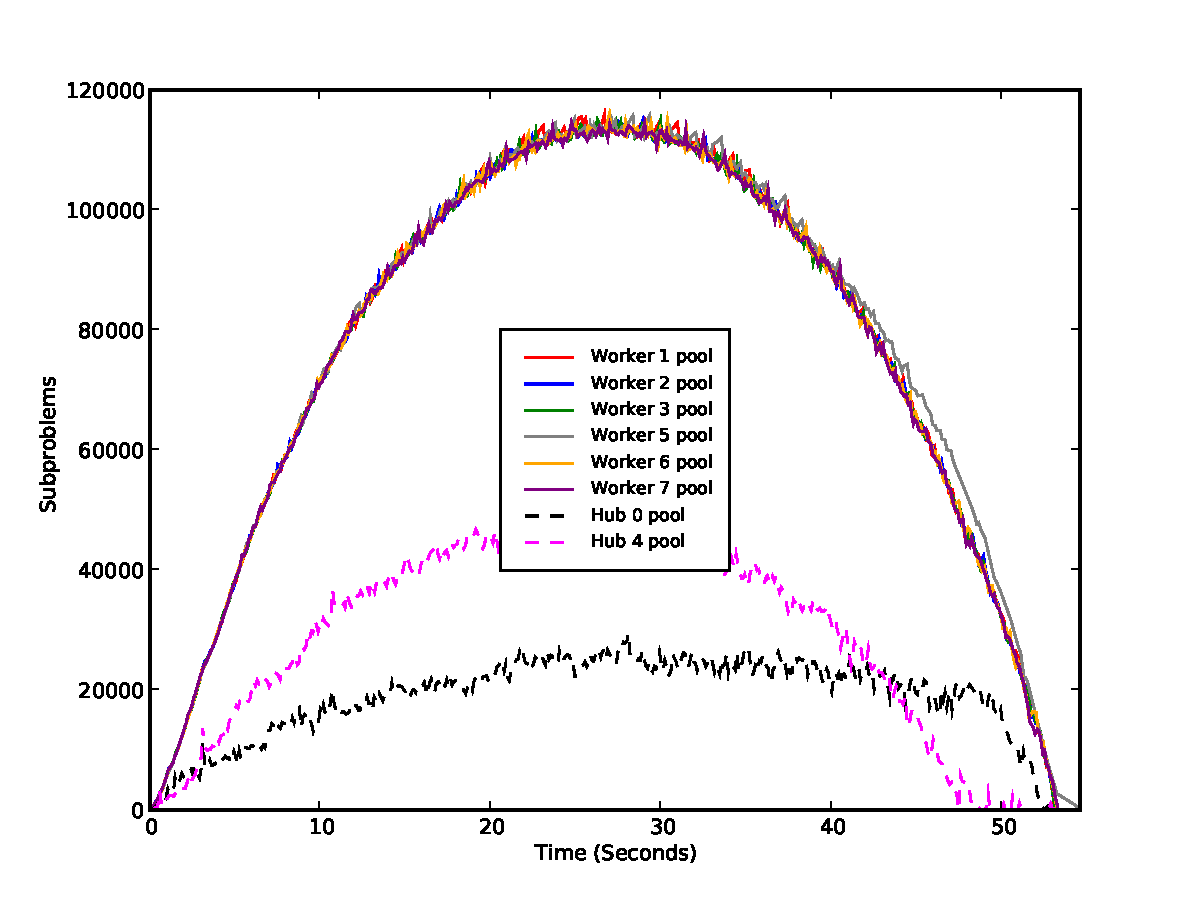
\includegraphics[width=0.95\textwidth]{sample-load-graph}
\vspace{-0.45in}
\end{center}
\caption{Sample graphical output from \texttt{pebblLoadGraph}}.
\label{fig:loadGraph}
\end{figure}





\section*{Acknowledgements}

This work was performed in part at Sandia National
Laboratories. Sandia is a multipurpose laboratory operated by Sandia
Corporation, a Lockheed-Martin Company, for the United States
Department of Energy under contract DE-AC04-94AL85000.  This work was
also supported in part by National Science Foundation Grant
CCR-9902092.


\bibliographystyle{abbrv}
\bibliography{pebbl}

\end{document}
